\documentclass[a4paper, 12pt]{article}
\usepackage{hyperref}
\usepackage{xcolor}
\usepackage{graphicx}
\usepackage{float}
\usepackage[export]{adjustbox}
\usepackage[english]{babel}
\usepackage[T1]{fontenc}
\usepackage{url}
\usepackage{import}
\usepackage{multirow}
\usepackage{color}
\usepackage{fancyhdr}
\usepackage{amssymb}
\usepackage{tabu}
\usepackage{listings}
\usepackage[margin=2.5cm]{geometry}
\usepackage{titling}
\usepackage{listingsutf8}
\usepackage[utf8]{inputenc}
\usepackage{mathtools}
\usepackage[numbered,framed]{matlab-prettifier}
\usepackage{amsmath}
\usepackage{animate}
\usepackage[labelformat=empty]{caption}
\usepackage{subfig}


\let\ph\mlplaceholder
\lstMakeShortInline"

\newcommand{\bnb}{\begin{nobreak}}
\newcommand{\enb}{\end{nobreak}}

\lstset{
	style              = Matlab-editor,
  	basicstyle         = \mlttfamily,
  	escapechar         = ",
  	mlshowsectionrules = true,
}

\title{\vspace{2cm}Elaborato di\\ \textbf{Calcolo Numerico}\\ Anno Accademico 2017/2018\vspace{1cm}}

\author
{Moncini Federico - \texttt{5936828}\\ Capecchi Tommaso - \texttt{5943118} }

\addto\captionsenglish{\renewcommand{\contentsname}{Capitoli}}

\begin{document}

\pagenumbering{Roman}
\lstset{inputencoding=latin1}
	
\maketitle

\newpage

\newpage

\tableofcontents
\newpage

\pagenumbering{arabic}
	
	\vspace{0.8cm}
\section{\textbf{Capitolo}}
\subsection{}
\large\noindent\fbox{
	\parbox{\textwidth}{
	Sia $x = e \approx 2.7183 = \tilde{x}$. Si calcoli il corrispondente errore relativo $\epsilon_{x}$
e il numero di cifre significative k con cui $\tilde{x}$ approssima x. Si verifichi
che \\
	\begin{center}
	$|\epsilon_{x}|\approx \frac{1}{2}{10}^{-k} $
	\end{center}
	}
}\\
\begin{flushleft}
	\large \textbf{Soluzione}\\[0.5cm]
	L'errore relativo è definito come $|\epsilon_{x}| = \frac{|x-\hat{x}|}{|x|}$ , dalla quale ricavo la $\hat{x}$ come segue:\\
	$\hat{x} = x(1+\epsilon_{x})$ e dunque $\frac{\hat{x}}{x} = 1+\epsilon_{x}$. Ciò ci suggerisce che l'errore relativo deve essere comparato a 1; esso sarà piccolo se si avvicina allo zero (ciò implica che il risultato approssimato sarà vicino al risultato esatto di un dato problema), viceversa un errore relativo vicino a 1 comporta una quasi totale perdita di informazione. Calcoliamo quindi l'errore relativo:
	\begin{center}
		$|\epsilon_{x}| = \frac{|e-2.7183|}{|e|} = 7.3576e - 06$
	\end{center}
	Calcoliamo adesso il numero di cifre significative, ricavabili dalla seguente formula $k \approx -\log_{10}(2|\epsilon_{x}|)$
	\begin{center}
		$k \approx -\log_{10}(2|\epsilon_{x}|) \Longrightarrow k \approx 4.8322 \approx 5$
	\end{center}
	Verifico ora che $|\epsilon_{x}|\approx \frac{1}{2}{10}^{-k} $. Infatti:
	\begin{center}
		$|\epsilon_{x}| \approx 5e-06$
	\end{center}
\end{flushleft}

\newpage
\subsection{}
\large\noindent\fbox{
	\parbox{\textwidth}{
	Usando gli sviluppi di Taylor fino al secondo ordine con resto in forma di Lagrange, si verifichi che se \(f \in C^3\), risulta 
	\begin{center}
		\(f'(x)=\phi_h(x)+O(h^2)\) dove \(\phi_h(x)=\frac{f(x+h)-f(x-h)}{2h}\).
	\end{center}
	}
}
\begin{flushleft}
	\large \textbf{Soluzione}\\[0.5cm]
	$f'(x) = \phi_{h}(x) + O(h^{2})$\\[0.3cm]
	$\phi_{h}(x) = \frac {f(x+h)-f(x-h)}{2h}$\\[0.3cm]
	Per mezzo degli sviluppi di Taylor fino al secondo ordine ottengo che:\\[0.3cm]
	$f(x) = f(x_{0})+ f'(x_{0})(x-x_{0})+\frac {f''(x_{0})}{2!}(x-x_{0})^{2}+O[(x-x_{0})^{3}$\\[0.3cm]
	Ricavo dunque $f(x+h)$ e $f(x-h)$:\\[0.3cm]
	$f(x+h) = f(x_{0})+ hf'(x_{0})+\frac{h^{2}}{2}f''(x^{2})+O(h^{3})$\\[0.3cm]
	$f(x-h) = f(x_{0})- hf'(x_{0})+\frac{h^{2}}{2}f''(x^{2})+O(h^{3})$\\[0.3cm]
	Ottengo quindi:
	$f'(x) = \frac{f(x_{0})+hf'(x_{0})+\frac{h^{2}}{2}f''(x_{0})+O(h^{3})-f(x_{0})+hf'(x_{0})-\frac{h^{2}}{2}f''(x_{0})+O(h^{3})}{2h}\Longrightarrow$\\[0.3cm]
	$f'(x) = \frac{2hf'(x_{0})+O(h^{3})}{2h} = f'(x_{0})+O(h^{2})$
\end{flushleft}
\newpage
\subsection{}
\large\noindent\fbox{
	\parbox{\textwidth}{
	Utilizzando Matlab, si costruisca una tabella dove, per $h = 10^{-j},j = 1,...,10$ e per la funzione $f(x) = x^{4}$ si riporta il valore di $\theta_{h}(x)$ definito nell'Esercizio 1 in x = 1. Commentare i risultati ottenuti.
	}
}
\begin{flushleft}
	\large \textbf{Soluzione}\\[0.5cm]
	Il seguente codice riguarda la soluzione dell'esercizio 3 con la relativa tabella dei risultati:
	\lstinputlisting[language=Matlab]{Codici/Cap1/Esercizio3.m}
	\begin{center}
		\begin{tabular}{|c|c|}
			\hline
				$h$ & $\theta_{h}(1)$ \\
			\hline
    			\(10^{-1}\) & $4.040000000000002$\\
    			\(10^{-2}\) & $4.000400000000004$\\
    			\(10^{-3}\) & $4.000003999999723$\\
    			\(10^{-4}\) & $4.000000039999230$\\
    			\(10^{-5}\) & $4.000000000403681$\\
    			\(10^{-6}\) & $3.999999999948489$\\
    			\(10^{-7}\) & $4.000000000115023$\\
    			\(10^{-8}\) & $4.000000003445692$\\
    			\(10^{-9}\) & $4.000000108916879$\\
    			\(10^{-10}\) & $4.000000330961484$\\
			\hline
		\end{tabular}
	\end{center}
	Come si nota dalla tabella, la funzione $f(x) = x^{4}$ decresce fino a $ i = 10^{-6}$ dopodiché cresce, come si puo notare anche dal seguente grafico:
	\begin{figure}[H]
	\label{Cap_1_Es_3}
	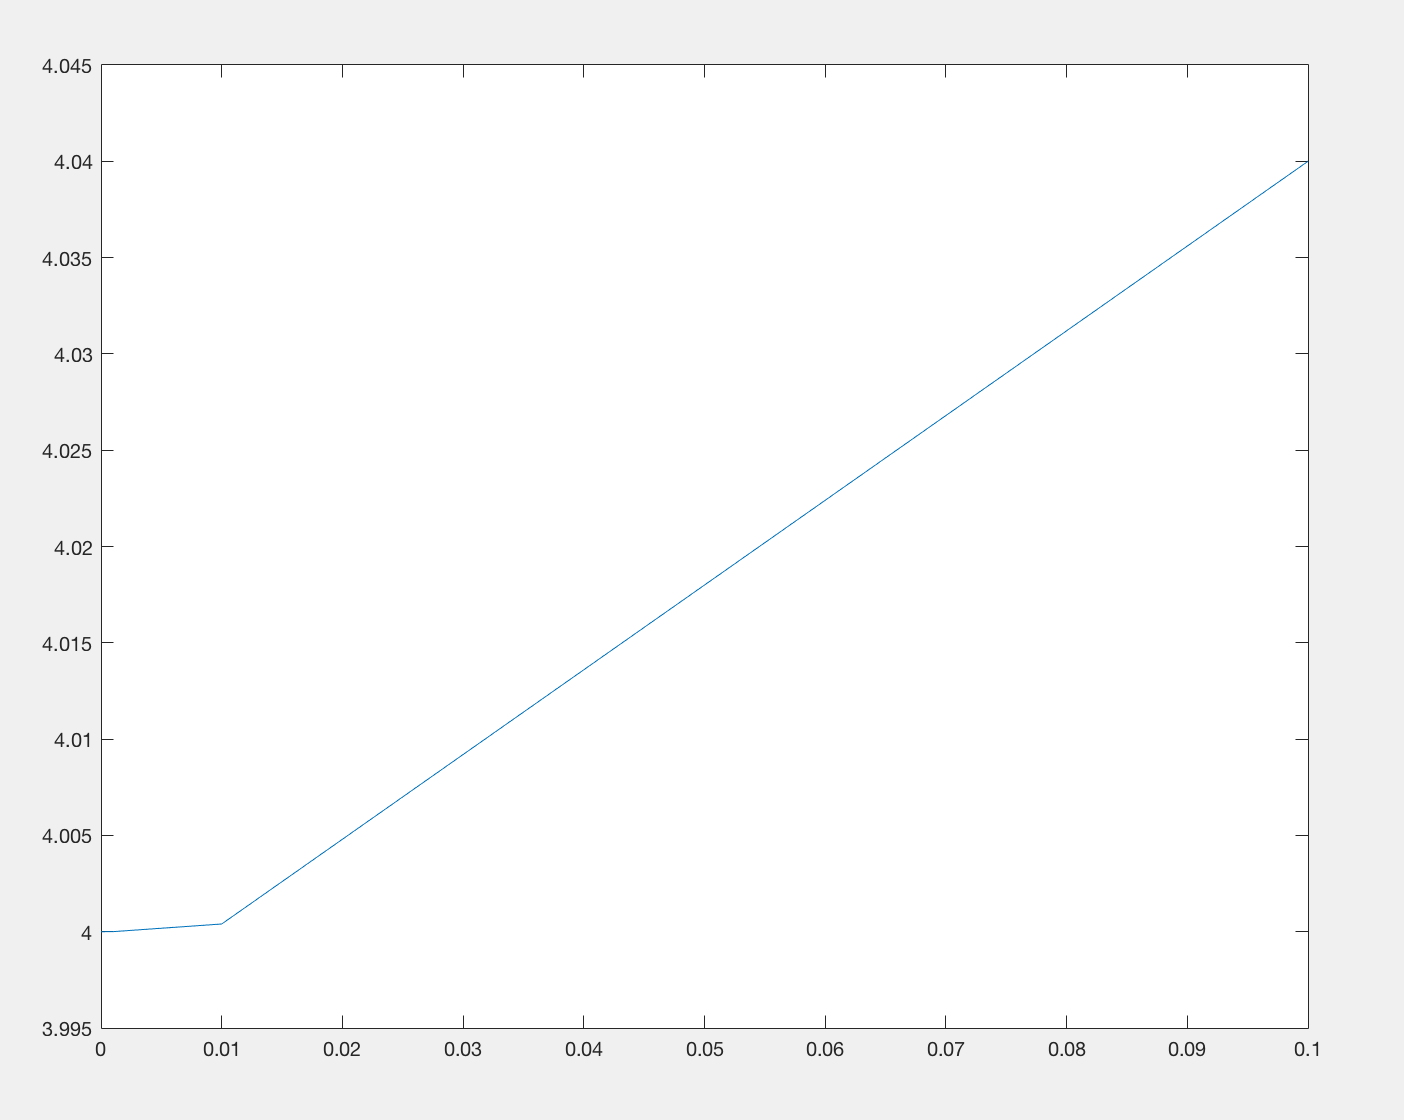
\includegraphics[width=\textwidth]{Codici/Cap1/Es3_Fig}
		\caption{Funzione $\theta_{h}(1)$}
	\end{figure}
\end{flushleft}
\newpage
\subsection{}
\large\noindent\fbox{
	\parbox{\textwidth}{
	Si dia una maggiorazione del valore assoluto dell'errore relativo con cui $x+y+z$ viene approssimato dall'approssimazione prodotta dal calcolatore, ossia $(x\oplus y)\oplus z$ (supporre che non ci siano problemi di overflow o di underflow). Ricavare l'analoga maggiorazione anche per $x\oplus (y\oplus z)$ tenendo presente che $x\oplus (y\oplus z)$ = $(x\oplus y)\oplus z$.
	}
}
\begin{flushleft}
	\large \textbf{Soluzione}\\[0.3cm]
	Ricavo la maggiorazione del valore assoluto dell'errore di $(x\oplus y)\oplus z$:\\[0.3cm]
	\begin{Large}$\epsilon = \frac{(1 + \epsilon_{2})[(1+\epsilon_{1})(x(1+\epsilon_{x})+y(1+\epsilon_{y}))+z(1+\epsilon_{z})]-(x+y+z)}{x+y+z}$ = \\[0.3cm]
	$\frac{(1+\epsilon_{2}) \{[(1+ \epsilon_{1})(x+x\epsilon_{x}+y+y\epsilon_{y})]+z+z\epsilon_{z}\}-x-y-z}{x+y+z}$ = \\[0.3cm]
	$\frac{(1+ \epsilon_{2})\{x+x\epsilon_{x}+y+y\epsilon_{y}+x\epsilon_{1}+x\epsilon_{x}\epsilon_{1}+y\epsilon_{1}+y\epsilon_{y}\epsilon_{1}+z+z\epsilon_{z}\}-x-y-z}{x+y+z}$\\[0.3cm]
	$\frac{(1+\epsilon_{2}\{x(1+\epsilon_{x}+\epsilon_{1}+\epsilon_{x}\epsilon_{1})+y(1+\epsilon_{y}+\epsilon_{1}+\epsilon_{y}\epsilon_{1})+z(1+\epsilon_{z})\}-x-y-z}{x+y+z}$\\[0.3cm]
	$\frac{(x+x\epsilon_{2})(1+\epsilon_{x}+\epsilon_{1}+\epsilon_{x}\epsilon_{1})+(x+y\epsilon_{2})(1+\epsilon_{y}+\epsilon_{1}+\epsilon_{y}\epsilon_{1})+(z+z\epsilon_{2})(1+\epsilon_{z})-x-y-z}{x+y+z}$\\[0.3cm]
	$\leq |\frac{x\epsilon_{x}+y\epsilon_{y}+z\epsilon_{z}+x\epsilon_{1}+y\epsilon_{1}+x\epsilon_{2}+y\epsilon_{2}+z\epsilon_{2}}{x+y+z}| =$
	$ |\frac{x\epsilon_{x}+y\epsilon_{y}+z\epsilon_{z}+\epsilon_{1}(x+y)+\epsilon_{2}(z+y+z)}{x+y+z}|$ \\[0.3cm]
	$\leq \frac{|x| |\epsilon_{x}| + |y| |\epsilon_{y} | + |z| |\epsilon_{z}| + |\epsilon_{1}| |x+y| + |\epsilon_{2}| |x+y+z|}{|x+y+z|}$ \\[0.3cm]
	$\leq \frac{\epsilon_{m}(|x|+|y|+|z|)+|x+y|+|x+y+z|}{|x+y+z|} = \epsilon_{m}(\frac{|x|+|y|+|z|}{|x+y+z|}+|\frac{|x+y|}{|x+y+z|}+1)$
	\end{Large}\\[0.3cm]
	Per ricavare la maggiorazione del valore assoluto dell'errore di $x\oplus (y\oplus z)$ è necessario scambiare al posto della x la lettera z, e si otterrà l'analoga maggiorazzione:\\[0.3cm]
	\begin{large}
		$\epsilon_{m}(\frac{|x|+|y|+|z|}{|x+y+z|}+|\frac{|z+y|}{|x+y+z|}+1)$\\[0.3cm]
		Otteniamo quindi che i valori degli errori $\varepsilon_{1}$ e $\varepsilon_{2}$ sono condizionati rispettivamente, dai valori $\frac{|x+y|}{|x+y+z|}$ e $\frac{|y+z|}{|y+z+x|}$.

	\end{large}
\end{flushleft}
\newpage
\subsection{}
\large\noindent\fbox{
	\parbox{\textwidth}{
	Eseguire le seguenti istruzioni in Matlab:
		\begin{center}
		x = 0; count = 0;\\
		$while x \sim 1$, x = x + delta, count = count + 1, end\\
		\end{center}
		dapprima ponendo $delta = \frac{1}{16}$ e poi ponendo $delta = \frac{1}{20}$. Commentare i risultati ottenuti e in particolare il non funzionamento del secondo caso.
	
	}
}
\begin{flushleft}
	\large \textbf{Soluzione}\\[0.3cm]
		\lstinputlisting[language=Matlab]{Codici/Cap1/esercizio5.m}
		$\bullet$ Analizziamo il caso in cui $delta = \frac{1}{16}$\\[0.5cm]
		Il programma termina correttamente poiche $delta = \frac{1}{16} = 0.0625$ e dopo 16 iterazioni il valore raggiunta da x è proprio 1, che rispecchia la condizione di uscita del ciclo while.\\[0.5cm]
		$\bullet$Analizziamo il caso in cui $delta = \frac{1}{20}$\\[0.5cm]
		In questo caso il programma non termina poiche il controllo sul ciclo while non viene verificato correttamente; infatti $delta = \frac{1}{20} = [0.05]_{10}$, che rappresentato in base 2 risulta $[0.00\overline{0011}]_{2} $. Questo fa si che l'operazione di somma ad ogni iterazione riguardi numeri periodici che essendo approssimati non raggiungeranno ma il valore x = 1, dunque il ciclo non terminerà mai. Una soluzione protrebbe essere quella di sostituire il controllo del while con uno piu efficiente, come: abs(x-1) > eps
\end{flushleft}
\newpage
\subsection{}
\large\noindent\fbox{
	\parbox{\textwidth}{
		Verificare che entrambe le seguenti successioni convergono a $\sqrt{3}$, (riportare le successive approssimazioni in una tabella a due colonne, una per ciascuna successione),\\
		\begin{center}
			\begin{Large}
			$x_{k+1} = \frac{(x_{k} + \frac{3}{x_{k}})}{2}, x_{0} = 3;$\\[0.3cm]
			$x_{k+1} = \frac{3+x_{k-1}x_{x}}{x_{k-1}+x_{k}}, x_{0} = 3; x_{1} = 2$\\[0.3cm]
			\end{Large}
		\end{center}
		Per ciascuna delle due successioni, dire quindi dopo quante iterazioni si ottiene un'approssimazione con un errore assoluto minore o uguale a $10^{-12}$ in valore assoluto.
	}
}
\begin{flushleft}
	\large \textbf{Soluzione}\\[0.3cm]
	\begin{Large}
	$\bullet x_{k+1} = \frac{(x_{k} + \frac{3}{x_{k}})}{2}, x_{0} = 3;$\\[0.3cm]
	\end{Large}
	\lstinputlisting[language=Matlab]{Codici/Cap1/Esercizio6.m}
	Il codice precedente restituisce i seguenti risultati: 
	\begin{center}
		\begin{tabular}{|c|c|c|}
			\hline
				$k$ & $x_{k}$&$\epsilon_{k} $\\
			\hline
    			$0$ & $3.000000000000000$ & $ \epsilon_{0} = 1.267949e+00$\\
    			$1$ & $2.00000000000000$ & $ \epsilon_{1} = 2.679492e-01$\\
    			$2$ & $1.750000000000000$ & $\epsilon_{2} = 1.794919e-02$\\
    			$3$ & $1.732143000000000$ & $\epsilon_{3} = 9.204957e-05$\\
    			$4$ & $1.732051000000000$ & $\epsilon_{4} = 2.445850e-09$\\
    			$5$ & $1.732051000000000$ & $\epsilon_{5} = 0e+00$\\
			\hline
		\end{tabular}
	\end{center}
	Si vede quindi che per k >= 5 si ha un errore assoluto che equivale a 0, ovvero una quantita  minore o uguale di $10^{-12}$\\[0.3cm]
	\begin{Large}
	$\bullet x_{k+1} = \frac{3+x_{k-1}x_{x}}{x_{k-1}+x_{k}}, x_{0} = 3; x_{1} = 2$\\[0.3cm]
	\end{Large}
	\lstinputlisting[language=Matlab]{Codici/Cap1/Esercizio6_2.m}
	Il codice precedente restituisce i seguenti risultati: 
	\begin{center}
		\begin{tabular}{|c|c|c|}
			\hline
				$k$ & $x_{k}$&$\epsilon_{k} $\\
			\hline
    			$0$ & $3.000000000000000$ & $ \epsilon_{0} = 1.267949e+00$\\
    			$1$ & $2.00000000000000$ & $ \epsilon_{1} = 2.679492e-01$\\
    			$2$ & $1.80000000000000$ & $\epsilon_{2} = 6.794919e-02$\\
			$3$ & $1.736842000000000$ & $\epsilon_{3} = 4.791298e-03$\\
    			$4$ & $1.732143000000000$ & $\epsilon_{4} = 9.204957e-05$\\
    			$5$ & $1.7320510000000$ & $\epsilon_{5} = 1.271372e-07$\\
			$6$ & $1.7320510000000$ & $\epsilon_{6} = 3.378631e-12$\\
			\hline
		\end{tabular}
	\end{center}
	Si vede quindi che per k >= 6 si ha un errore assoluto che equivale a 0, ovvero una quantita  minore o uguale di $10^{-12}$\\[0.3cm]
	\end{flushleft}
\newpage
	\newpage
	\vspace{0.8cm}
\section{\textbf{Capitolo}}
\subsection{}
\large\noindent\fbox{
	\parbox{\textwidth}{
	Determinare analiticamente gli zeri del polinomio $P(x)=x^3 -4x^2 + 5x -2$ e la loro molteplicità.
	Dire perchè il metodo di bisezione è utilizzabile per approssimarne uno a partire dall’intervallo di confidenza \textit{[a , b] = [0 , 3]}. A quale zero di \textit{P} potrà tendere la successione generata dal metodo di bisezione a partire da tale intervallo? Costruire una tabella in cui si riportano il numero di iterazioni e di valutazioni di P richieste per valori decrescenti della tolleranza tolx.
	}}

Studio analitico del polinomio $P(x) = x^3-4x^2+5x-2$.\\
\begin{itemize}
	\item \textbf{Zeri del polinomio}\\
		Per trovare gli zeri del polinomio occorre scomporlo nel seguente modo:
			\[
			\ x^3-4x^2+5x-2 =
			\] 
			\[
			\ = (x-2)(x^2-2x+1) =
			\]
			\[
			\ = (x-2)(x-1)^2
			\]\\
		Da cui si deduce che $P(x)=0$ per $(x-2)=0 \Rightarrow x=2$ e $(x-1)=0 \Rightarrow x=1$. \\
	\item \textbf{Molteplicità}\\
		I valori di \textit{x} precedentemente calcolati vengono definiti come \textit{radici} del polinomio. Si dice che \textit{a} è una radice di \textit{P(x)} con \textit{molteplicità n} se e solo se \textit{P(x)} è divisibile per $(x-a)^n$, ma non è divisibile per $(x-a)^{n-1}$.\\
		Inoltre si dice che \textit{x} ha \textit{molteplicità esatta} $n \geq 1$, se:
			\[
			f(x) = f'(x) = ... = f^{(n-1)}(x) = 0,  f^{(n)}(x) \neq 0.
			\]
				$\bullet x = 2 $ \\[0.5cm]
					\[
					P(2) = 8-16+10-2 = 0 
					\]
					\[
					P'(2) = 3x^2-8x+5 = 12-16+5 = 1 \neq 0 \Rightarrow \textit{ molteplicità } n=1
					\]\\
				$\bullet x = 2 $ \\[0.5cm]
					\[
					P(1) = 1-4+5-2 = 0 
					\]
					\[
					P'(1) = 3x^2-8x+5 = 3-8+5 = 0 
					\]
					\[
					P''(1) = 6x-8 = 6-8 \neq 0 \Rightarrow \textit{ molteplicità } n=2
					\]
		In questo caso la radice $x=2$ viene definita \textit{semplice} in quanto ha molteplicità $m=1$,
mentre la radice $x=1$ si definisce \textit{multipla} data la molteplicità $m=2$.\\ 
\end{itemize}
Il requisito per poter applicare il \textit{metodo di bisezione} in un intervallo $[a,b]$ è che sia $f(a)f(b)<0$ in modo da garantire l'esistenza di almeno uno zero. Per il polinomio $P(x)$ è possibile applicare il \textit{metodo di bisezione} nell'intervallo $[0,3]$ poichè il requisito è soddisfatto.
In questo caso si ha: $P(0)*P(3) = (-2)*(4) = -8$.\\\\
Il seguente codice MatLab, riguarda il \textbf{Metodo di bisezione}:\\
	\lstinputlisting[language=Matlab]{Codici/Cap2/Bisezione_Es1.m}
Nel seguente codice Matlab viene applicato il \textit{metodo di bisezione} al polinomio $P(x)$ sull'intervallo $[0,3]$, con una tolleranza iniziale pari a $10^-1$, la quale viene decremntata di un fattore $10$ ad ogni iterazione:\\
	\lstinputlisting[language=Matlab]{Codici/Cap2/Es1_cap2.m}
Da i seguenti valori riportati dall'esecuzione del codice è possibile notare che la successione generata dal metodo di \textit{bisezione} converge alla radice $x = 2$:\\
\begin{center}
	\begin{tabular}{|c|c|c|}
		\hline
			$tol_x$ & \textit{Bisezione} & \textit{Num. Iterazioni} \\
		\hline
   			$10^{-1}$ & $\tilde{x} = 1.500000000000000$ & $ib = 0$\\
    		$10^{-2}$ & $\tilde{x} = 1.992187500000000$ & $ib = 6$\\
    		$10^{-3}$ & $\tilde{x} = 2.000976562500000$ & $ib = 9$\\
    		$10^{-4}$ & $\tilde{x} = 2.000061035156250$ & $ib = 13$\\
   			$10^{-5}$ & $\tilde{x} = 1.999992370605469$ & $ib = 16$\\
   			$10^{-6}$ & $\tilde{x} = 2.000000953674316$ & $ib = 19$\\
    		$10^{-7}$ & $\tilde{x} = 2.000000059604645$ & $ib = 23$\\
    		$10^{-8}$ & $\tilde{x} = 1.999999992549419$ & $ib = 26$\\
    		$10^{-9}$ & $\tilde{x} = 2.000000000931323$ & $ib= 29$\\
    		$10^{-10}$ & $\tilde{x} = 2.000000000058208$ & $ib = 33$\\
    		$10^{-11}$ & $\tilde{x} = 1.999999999992724$ & $ib = 36$\\
    		$10^{-12}$ & $\tilde{x} = 2.000000000000910$ & $ib = 39$\\
    		$10^{-13}$ & $\tilde{x} = 2.000000000000057$ & $ib = 43$\\
    		$10^{-14}$ & $\tilde{x} = 1.999999999999993$ & $ib = 46$\\
    		$10^{-15}$ & $\tilde{x} = 2.000000000000001$ & $ib = 49$\\
		\hline
	\end{tabular}
\end{center}
\newpage
\subsection{}
\large\noindent\fbox{
	\parbox{\textwidth}{
	Scrivere una function Matlab che implementi la formula composita di Simpson su $2n + 1$ ascisse equidistanti nell’intervallo \textit{[a, b]}, relativamente alla funzione implementata da \textbf{fun(x)}. La function deve essere del tipo: \textbf{If = simpcomp( n, a, b, fun )}.
}}\\[0.5cm]

Il codice riportato in seguito implementa la formula \textit{composita di Simpson} su $2n+1$ ascisse
equidistanti definite sull'intervallo \textit{[a,b]}, relativa alla generica funzione $fun(x)$ e ne 
restiusce l'approssimazione del relativo integrale.
\lstinputlisting[language=Matlab]{Codici/Cap5/simpcomp.m}
\newpage
\subsection{}
\large\noindent\fbox{
	\parbox{\textwidth}{
	Scrivere una function Matlab che implementi la formula composita dei trapezi adattativa nell’intervallo \textit{[a, b]}, relativamente alla funzione implementata da \textbf{fun(x)}, e con tolleranza \textbf{tol}. La function deve essere del tipo:
	\textbf{If = trapad( a, b, fun, tol )}.
}}\\[0.5cm]

Il codice riportato in seguito implementa la formula \textit{adattiva dei trapezi} sull'intervallo  \textit{[a,b]},
relativa alla generica funzione fun(x), con una tolleranza tol e ne 
restiusce l'approssimazione del relativo integrale.\\
\lstinputlisting[language=Matlab]{Codici/Cap5/trapad.m}
\newpage
\subsection{}
\large\noindent\fbox{
	\parbox{\textwidth}{
	Definire una procedura iterativa basata sul metodo di Newton per approssimare $\sqrt{\alpha}$, per un assegnato $\alpha > 0$. Costruire una tabella dove si riportano le successive approssimazioni ottenute e i corrispondenti errori assoluti (usare l’approssimazione Matlab di $\sqrt{\alpha}$ per il calcolo dell’errore) nel caso in cui $\sqrt{\alpha} = 5$ partendo da $x_{0} = 5$.
	}}\\

Dato che  $\sqrt{\alpha}$ è la radice ricercata, occorre quindi trovare una
funzione $f(x)$ che abbia uno \textit{zero} in appunto $\sqrt{\alpha}$.
La funzione ricercata in questo caso è $f(x) = x^2 - \alpha$, la quale ha due radici
semplici in $\pm\sqrt{\alpha}$ e ha derivata $f'(x) = 2x$.\\\\
L'iterazione del metodo di Newton utilizzando questa funzione diventa :
	\[
	x_{i+1} = x_i-\frac{f(x_i)}{f'(x_i)} = x_i - \frac{x_i^2-\alpha}{2x_i} =
	\]
	\[
	= \frac{2x_i^2-x_i^2+\alpha}{2x_i} = \frac{x_i^2+\alpha}{2x_i} =
	\]
	\[
	= \frac{1}{2} \Bigl( x_i+\frac{\alpha}{x_i} \Bigl),\quad i=0,1,2,...
	\]\\\\
Il seguente codice MatLab, riguarda l'implementazione del \textbf{metodo di Newton per il calcolo} $\sqrt{\alpha}$:\\ 
	\lstinputlisting[language=Matlab]{Codici/Cap2/newtonSolveEs4.m}
Il seguente codice MatLab, riguarda la chiamata della funzione definita precedentemente, con $\alpha=x_0=5$, con numero di passi massimi $itmax=10$ e indice di tolleranza $tol_x=eps$ :\\
	\lstinputlisting[language=Matlab]{Codici/Cap2/Es4_cap2.m}
restituisce i seguenti valori:\\
\begin{center}
	\begin{tabular}{|c|c|c|}
		\hline
			$i$ & $x_i$ & $E_{ass}=\epsilon_i=|x_i-\sqrt{\alpha}| \quad \alpha=5$ \\
		\hline
    		$i=0$ & $x_0 = 5$ & $|\epsilon_0| = 2.763932022500210$\\
    		$i=1$ & $x_1 = 3$ & $|\epsilon_1| = 0.763932022500210$\\
    		$i=2$ & $x_2 = 2.333333333333334$ & $|\epsilon_2| = 0.097265355833544$\\
    		$i=3$ & $x_3 = 2.238095238095238$ & $|\epsilon_3| = 0.002027260595448$\\
    		$i=4$ & $x_4 = 2.236068895643363$ & $|\epsilon_4| = 9.181435736138610e-07$\\
    		$i=5$ & $x_5 = 2.236067977499978$ & $|\epsilon_5| = 1.882938249764266e-13$\\
    		$i=6$ & $x_6 = 2.236067977499790$ & $|\epsilon_6| = 0$\\
    		$i=7$ & $x_7 = 2.236067977499790$ & $|\epsilon_7| = 0$\\
		\hline
	\end{tabular}
\end{center}
\newpage
\subsection{}
\large\noindent\fbox{
	\parbox{\textwidth}{
	Definire una procedura iterativa basata sul metodo delle secanti sempre per approssimare $\sqrt{\alpha}$, per un assegnato $\alpha > 0$. Completare la tabella precedente aggiungendovi i risultati ottenuti con tale procedura partendo da $x_{0} = 5$ e $x_{1} = 3$. Commentare i risultati riportati in tabella.
	}}\\

Come visto nel precedente esercizio occorre utilizzare la funzione $f(x) = x^2 - \alpha$\\
L'iterazione del metodo delle Secanti utilizzando questa funzione diventa:
	\[
	x_{i+1} = \frac{f(x_i)x_{i-1}-f(x_{i-1})x_i}{f(x_i)-f(x_{i-1})} =
	\]
	\[
	= \frac{(x_i^2-\alpha)x_{i-1}-(x_{i-1}^2-\alpha)x_i}{x_i^2-\alpha-x_{i-1}^2+\alpha}  =
	\]
	\[
	= \frac{x_i^2x_{i-1}-\alpha x_{i-1}-x_{i-1}^2x_i+\alpha x_i}{x_i^2-x_{i-1}^2} =
	\]
	\[
	= \frac{x_ix_{i-1}(x_i-x_{i-1})+\alpha (x_i-x_{i-1})}{(x_i-x_{i-1})(x_i+x_{i-1})} =
	\]
	\[
	= \frac{(x_i-x_{i-1})(x_ix_{i-1}+\alpha)}{(x_i-x_{i-1})(x_i+x_{i-1})} =
	\]
	\[
	= \frac{x_ix_{i-1}+\alpha}{x_i+x_{i-1}},\quad i=0,1,2,...
	\]\\
L'implementazione del metodo delle secanti in Matlab è la seguente:\\ 
	\lstinputlisting[language=Matlab]{Codici/Cap2/secantiSolveEs5.m}
Il seguente codice MatLab, riguarda la chiamata della funzione definita precedentemente, con $\alpha=x_0=5$, con $x_1=3$, con numero di passi massimi $imax=100$ e indice di tolleranza $tol_x=eps$ :\\
	\lstinputlisting[language=Matlab]{Codici/Cap2/Es5_Cap2.m}
restituisce i seguenti valori:\\
\begin{center}
	\begin{tabular}{|c|c|c|}
		\hline
			$i$ & $x_i$ & $E_{ass}=\epsilon_i=|x_i-\sqrt{\alpha}| \quad \alpha=5$ \\
		\hline
    		$i=0$ & $x_0 = 5$ & $|\epsilon_0| = 2.763932022500210$\\
    		$i=1$ & $x_1 = 3$ & $|\epsilon_1| = 0.763932022500210$\\
    		$i=2$ & $x_2 = 2.500000000000000$ & $|\epsilon_2| = 0.263932022500210$\\
    		$i=3$ & $x_3 = 2.272727272727273$ & $|\epsilon_3| = 0.36659295227483$\\
    		$i=4$ & $x_4 = 2.238095238095238$ & $|\epsilon_4| = 0.00202760595448$\\
    		$i=5$ & $x_5 = 2.236084452975048$ & $|\epsilon_5| = 1.647547525829296e-05$\\
    		$i=6$ & $x_6 = 2.236067984964863$ & $|\epsilon_6| = 7.465073448287285e-09$\\
    		$i=7$ & $x_7 = 2.236067977499817$ & $|\epsilon_7| = 2.753353101070388e-14$\\
    		$i=8$ & $x_8 = 2.236067977499790$ & $|\epsilon_8| = 4.440892098500626e-16$\\
    		$i=9$ & $x_9 = 2.236067977499790$ & $|\epsilon_9| = 0$\\
    		$i=10$ & $x_{10} = 2.236067977499790$ & $|\epsilon_{10}| = 0$\\
		\hline
	\end{tabular}
\end{center}
\newpage
	\newpage
	\vspace{0.8cm}
\section{\textbf{Capitolo}}
\subsection{}
\large\noindent\fbox{
	\parbox{\textwidth}{
	Scrivere una function Matlab per la risoluzione di un sistema lineare con matrice dei coefficienti triangolare inferiore a diagonale unitaria. Inserire un esempio di utilizzo.
	}
}
\begin{flushleft}
	\large \textbf{Soluzione}\\[0.5cm]
	Il seguente codice riguarda la risoluzione di un sistema triangolare inferiore a diagonale unitaria:
	\lstinputlisting[language=Matlab]{Codici/Cap3/trisolveInf.m}
	Un esempio di utilizzo è dato dalla seguente matrice A, e vettore dei termini noti b:\\
		\begin{center}
			$A = \begin{bmatrix}
				1 & 0 & 0\\
				2 & 1 & 0\\
				3 & 2 & 1
			\end{bmatrix}\quad
			b = \begin{bmatrix}
				1\\
				2\\
				3\end{bmatrix}$\\
				E si ottiene il seguente vettore soluzione:
					$x = \begin{bmatrix}
					1\\
					0\\
					0\end{bmatrix}$\\
			\end{center}
\end{flushleft}
\newpage
\subsection{}
\large\noindent\fbox{
	\parbox{\textwidth}{
	Utilizzare l'Algoritmo 3.6 del libro per stabilire se le seguenti matrici sono sdp o no,
	\begin{center}
		$A_{1} = \begin{bmatrix}
				1 & -1 & 2 & 2\\
				-1 & 5 & -14 & 2\\
				2 & -14 & 42 & 2\\
				2 & 2 & 2 & 65
			\end{bmatrix}$,
			$A_{2} = \begin{bmatrix}
				1 & -1 & 2 & 2\\
				-1 & 6 & -17 & 3\\
				2 & -17 & 48 & -16\\
				2 & 3 & -16 & 4
			\end{bmatrix}$
	\end{center}
	}
}
\begin{flushleft}
	\large \textbf{Soluzione}\\[0.5cm]
	L'algoritmo utilizzato per risolvere l'esercizio è quello della fattorizzazione $LDL^{T}$. Questo perchè grazie al Teorema 3.6 del libro, è noto che una matrice è sdp se e solo se questa è fattorizzabile $LDL^{T}$.\\Si riporta dunque il codice Matlab di tale fattorizzazione:
	\lstinputlisting[language=Matlab]{Codici/Cap3/LDLTFatt.m}
	$\bullet A_{1}$\\[0.3cm]
	Si richiama il precedente Algoritmo con la matrice $A_{1}$ come input. Si ottiene il seguente risultato:
	\begin{center}
		$A_{1} = \begin{bmatrix}
				1 & -1 & 2 & 2\\
				-1 & 4 & -14 & 2\\
				2 & -3 & 2 & 2\\
				2 & 1 & 5 & 7
			\end{bmatrix}$
		\end{center}
		\newpage
		$\bullet A_{2}$\\[0.3cm]
	Si richiama il precedente Algoritmo con la matrice $A_{2}$ come input. In questo caso però la matrice non risulta essere fattorizzabile $LDL^{T}$ e dunque l'esecuzione stamperà il seguente errore:\\[0.4cm]
		\textbf{Error using LDLTFatt (line 19)}\\	
		\textbf{Matrice non sdp}\\
	\end{flushleft}
\newpage
\subsection{}
\large\noindent\fbox{
	\parbox{\textwidth}{
	Scrivere una function Matlab che, avendo in ingresso un vettore \textbf{b} contenente i termini noti del sistema lineare \textbf{Ax = b} con A sdp e l'output dell'Algoritmo 3.6 del libro (matrice A riscritta nella porzione triangolare inferiore con i fattori L e D della fattorizzazione $LDL^{t}$ di A), ne calcoli efficientemente la soluzione.
	}
}
\begin{flushleft}
	\large \textbf{Soluzione}\\[0.5cm]
	Si vuole quindi risolvere il sistema Ax = b con A = $LDL^{t}$. Il seguente codice risolve tale sistema lineare efficientemente:
	\lstinputlisting[language=Matlab]{Codici/Cap3/solveLDLT.m}
	Si fattorizza la matrice A di modo che questa venga riscritta nella porzione triangolare inferiore con i fattori L e D della fattorizzazione $LDL^{t}$. Dopo di che per risolvere il sistema Ax = b, ci riconduciamo a risolvere i seguenti sistemi lineari:\\[0.3cm]
	$\bullet Ly = b$\\[0.1cm]
	Si impiega l'algoritmo di risoluzione per matrici triangolari inferiori precedentemente utilizzato. Vale la pena notare che per estrarre la parte triangolare inferiore a diagonale unitaria si utilizza la funzione tril((A,-1) che restituisce sotto matrice strettamente inferiore rispetto alla diagonale e la si concatena con una matrice identità che permette cosi di ricostruire una matrice triangolare inferiore a diagonale unitaria.\\[0.3cm]
	$\bullet Dz = y$\\[0.1cm]
	Si calcola la soluzione del sistema dividendo ogni elemento di x (soluzione del precedente sistema) con il vettore riga contenente gli elementi della diagonale di A\\[0.3cm]
	$\bullet L^{t} = z$\\[0.1cm]
	Infine per ottenere la soluzione finale si ricava dalla matrice A la sotto matrice triangolare inferiore a diagonale unitaria con la stessa tecnica precedentemente utilizzata, calcolandone però la trasposta di modo da ricavare la sotto matrice triangolare superiore. Si invoca il seguente algoritmo per la sua risoluzione:
	\lstinputlisting[language=Matlab]{Codici/Cap3/trisolvesup.m}
	\end{flushleft}
\newpage
\subsection{}
\large\noindent\fbox{
	\parbox{\textwidth}{
	Scrivere una function Matlab che, avendo in ingresso un vettore \textbf{b} contenente i termini noti del sistema lineare \textbf{Ax = b} con A sdp e l'output dell'Algoritmo 3.7 del libro (matrice A riscritta con la fattorizzazione LU con pivoting parziale e il vettore \textbf{p} delle permutazioni), ne calcoli efficientemente la soluzione.
	}
}
\begin{flushleft}
	\large \textbf{Soluzione}\\[0.5cm]
	Con il seguente codice Matlab si ricava la fattorizzazione A = LU con pivoting parziale
	\lstinputlisting[language=Matlab]{Codici/Cap3/LUPivoting.m}
	Si vuole risolvere il sistema Ax = b con A = LU. Per farlo utilizziamo il codice:
	\lstinputlisting[language=Matlab]{Codici/Cap3/LUPivotingSolve.m}
	La soluzione sarà data quindi dalla risoluzione dei due sistemi lineari:\\[0.3cm]
	$\bullet Ly = b$\\[0.1cm]
	Si ricava dalla matrice A la sotto matrice triangolare inferiore a diagonale unitaria e si risolve tale sistema per mezzo dell'algoritmo di risoluzione \textbf{trisolveInf(A,b)}\\[0.3cm]
	$\bullet Ux = y$\\[0.1cm]
	Si ricava dalla matrice A la sotto matrice triangolare superiore e si risolve tale sistema per mezzo dell'algoritmo di risoluzione \textbf{trisolveSup(A,b)}\\[0.3cm]
	\end{flushleft}
\newpage
\subsection{}
\large\noindent\fbox{
	\parbox{\textwidth}{
	Inserire alcuni esempi di utilizzo delle due function implementate per i punti 3 e 4, scegliendo per ciascuno di essi un vettore $\hat{x}$ e ponendo \textbf{b = A$\hat{x}$}. Riportare $\hat{x}$ e la soluzione \textbf{x} da essi prodotta. Costruire anche una tabella in cui, per ogni esempio considerato, si riportano il numero di condizionamento di A in norma 2 (usare cond di Matlab) e le quantità $\|r\|/\|b\|$ e $\|x-\hat{x}\|/\|\hat{x}\|$.
	}
}
\begin{flushleft}
	\large \textbf{Soluzione}\\[0.5cm]
	Si riporta in seguito il codice utilizzato per la risoluzione del problema. Questo contiene le chiamate delle funzioni precedentemente descritte nell'esercizio 3 e 4:
	\lstinputlisting[language=Matlab]{Codici/Cap3/soluzioneEs5Cap3.m}
	$\bullet$ Esempio esercizio 3 ($A = LDL^{t}$)\\[0.1cm]
		\begin{center}
			$A = \begin{bmatrix}
				11 & 4 & -2\\
				6 & 7 & -1\\
				5 & 1 & 12
			\end{bmatrix}$, 
			$\hat{x} = \begin{bmatrix}
				64\\
				8\\
				13
			\end{bmatrix}$, 
			$A\hat{x} = b = \begin{bmatrix}
				710\\
				427\\
				484
			\end{bmatrix}$\\[0.1cm]
			\end{center}
			Dalla fattorizzazione A = $LDL^{t}$ ottengo:\\[0.5cm]
			\begin{center}
			$L = \begin{bmatrix}
				1 & 0 & 0\\
				0.5455 & 1 & 0\\
				0.4545 & -0.4634 & 1
			\end{bmatrix}$,
			$D = \begin{bmatrix}
				11 & 0 & 0\\
				0 & 3.7273 & 0\\
				0 & 0 & 8.9268
			\end{bmatrix}$,
			$L^{t} = \begin{bmatrix}
				1 & 0.5455 & 0.4545\\
				0 & 1 & -0.4634\\
				0 & 0 & 1
			\end{bmatrix}$\\[0.3cm]
			\end{center}
			\newpage
			Dalla quale ricavo la soluzione:\\[0.5cm]
			\begin{center}
			$x = \begin{bmatrix}
				44.4945\\
				19.9863\\
				20.1284
			\end{bmatrix}$
			\end{center}
			$\bullet$ Esempio esercizio 4 (A = LU con pivoting)\\[0.1cm]
			\begin{center}
			$A = \begin{bmatrix}
				11 & 4 & -2\\
				6 & 7 & -1\\
				5 & 1 & 12
			\end{bmatrix}$, 
			$\hat{x} = \begin{bmatrix}
				64\\
				8\\
				13
			\end{bmatrix}$, 
			$A\hat{x} = b = \begin{bmatrix}
				710\\
				427\\
				484
			\end{bmatrix}$\\[0.1cm]
			\end{center}
			Dalla fattorizzazione A = LU con pivoting, si ottiene:\\[0.5cm]
			\begin{center}
			$L = \begin{bmatrix}
				1 & 0 & 0\\
				0.5455 & 1 & 0\\
				0.4545 & -0.1698 & 1
			\end{bmatrix}$,
			$U = \begin{bmatrix}
				11 & 4 & -2\\
				0 & 4.8182 & 0.0909\\
				0 & 0 & 12.9245
			\end{bmatrix}$\\[0.5cm]
			In questo caso non vengono effettuati scambi tra le righe, dunque il vettore b rimane invariato.
			Si ottiene quindi il risultato:\\[0.5cm]
			$x = \begin{bmatrix}
				64\\
				8.000000000000004\\
				13.000000000000004
			\end{bmatrix}$\\[0.5cm]
			\end{center}
			Di seguito si riporta in una tabella il numero di condizionamento di A in norma 2 e le quantità $\|r\|/\|b\|$ e $\|x-\hat{x}\|/\|\hat{x}\|$.\\[0.5cm]
			\begin{center}
				\begin{tabular}{| c | c | c | c |}
					\hline
						\textit{A} & $K_2(A)$ & $\frac{\|r\|}{\|b\|}$ & $\frac{\|x-\hat{x}\|}{\|\hat{x}\|}$ \\
					\hline
						$A= LDL^{t}$ & 4.1947 & 0.1931 & 0.3644\\
						$A= LU$ & 4.1947 & 5.9241e-17 & 7.6363e-17\\
					\hline
				\end{tabular}
			\end{center}
\end{flushleft}
\newpage
\subsection{}
\large\noindent\fbox{
	\parbox{\textwidth}{
	Sia $A = \begin{bmatrix}
				\epsilon & 1\\
				1 & 1
			\end{bmatrix}$ con $\epsilon = 10^{-13}$. Definire L triangolare inferiore a diagonale unitaria e U triangolare superiore in modo che il prodotto LU sia la fattorizzazione LU di A e, posto b = Ae, con $e = (1,1)^{T}$, confrontare l'accuratezza della soluzione che si ottiene usando il comando $U \backslash(L \backslash b)$ (Gauss senza pivoting) e il comando $A \backslash b $(Gauss con pivoting),
	}
}
\begin{flushleft}
	\large \textbf{Soluzione}\\[0.5cm]
	Con il seguente codice si effettua la fattorizzazione A = LU:
	\lstinputlisting[language=Matlab]{Codici/Cap3/luFactorization.m}
	Si richiama inoltre il seguente codice Matlab per effettuare la chiamata alla funzione $luFactorization(A)$, ricavare quindi la sottomatrice triangolare inferiore a diagonale unitaria (L) e la sottomatrice triangolare superiore (U); si assegna a b la quantità Ae ed infine si confrontano i risultati usando prima Gauss senza pivoting e poi Gauss con pivoting.
	\lstinputlisting[language=Matlab]{Codici/Cap3/SoluzioneEs6Cap3.m}
	Dalla fattorizzazione si ottiene:\\[0.5cm]
	\begin{center}
	$A = \begin{bmatrix}
				1.0000e-13 & 1\\
				1.0000e+13 & -1.0000e+13
			\end{bmatrix}$,
			$L = \begin{bmatrix}
				1& 0\\
				1.0000e+13 & 1
			\end{bmatrix}$,
			$U = \begin{bmatrix}
				1.0000e-13 & 1\\
				0 & -1.0000e+13
			\end{bmatrix}$\\[0.5cm]
			\end{center}
			Calcolando il vettore b = Ae si ottiene:\\[0.5cm]
			\begin{center}
			$ b = \begin{bmatrix}
				1.000000000000100\\
				1
			\end{bmatrix}$\\[0.5cm]
			Infine si ottengono i due vettori rispettivamente di Gauss senza pivoting e Gauss con pivoting:\\[0.5cm]
			$ gSp = \begin{bmatrix}
				0\\
				1.000000000000100
			\end{bmatrix}$, 
			$ gp = \begin{bmatrix}
				1\\
				1
			\end{bmatrix}$
			\end{center}
			Dunque si nota come Gauss con pivoting sia piu accurato rispetto a Gauss senza pivoting.
	\end{flushleft}
	
\newpage
\subsection{}
\large\noindent\fbox{
	\parbox{\textwidth}{
	Scrivere la function Matlab specifica per la risoluzione di un sistema lineare con matrice dei coefficienti $A \in R^{nxn}$ bidiagonale inferiore a diagonale unitaria di Toeplitz, specificabile con uno scalare $\alpha$. Sperimentarne e commentarne le prestazioni (considerare il numero di condizionamento della matrice) nel caso in cui $n$ = 12 e $\alpha = 100$ ponendo dapprima $b = (1,101,...101)^{T}$ (soluzione esatta $\hat{x} = (1,...,1)^{T})$ e quindi b = 0.1 * $(1,101,...,101)^{T})$ (soluzione esatta $\hat{x} = (0.1,...,0.1)^{T}$).
	}
}
\begin{flushleft}
	\large \textbf{Soluzione}\\[0.5cm]
	Si riporta in seguito il codice utilizzato per la risoluzione di un sistema lineare Ax = b, con $A \in R^{nxn}$ bidiagonale inferiore a diagonale unitaria di Toeplitz, che ha la seguente forma:
	\begin{center}
	$A = \begin{bmatrix}
				1 & 0 & \ldots & \ldots & 0\\
				\alpha & 1 & 0 & \ldots & 0\\
				0 & \ddots & \ddots & \ddots & \vdots\\
				\vdots & \ddots & \ddots & \ddots & \vdots\\
				0 & \ldots & \ldots & \alpha & 1
			\end{bmatrix}$\\[0.5cm]
	\end{center}
	\lstinputlisting[language=Matlab]{Codici/Cap3/trisolveInfAlphaToeplitz.m}
	Il seguente codice invece riguarda la soluzione dell'esercizio:
	\lstinputlisting[language=Matlab]{Codici/Cap3/SoluzioneEs7Cap3.m}
	\newpage
	Si ottengono quindi i due vettori soluzione:\\[0.5cm]
	\begin{center}
	$x = \begin{bmatrix}
				1\\
				1\\
				1\\
				1\\
				1\\
				1\\
				1\\
				1\\
				1\\
				1\\
				1\\
				1\\
			\end{bmatrix}$,
			$x1 = \begin{bmatrix}
				1.0000000000000000e-01\\
				1.0000000000000014e-01\\
				9.999999999985931e-02\\
				1.000000000140702e-01\\
				9.999999859298470e-02\\
				1.000001407015319e-01\\
				9.998592984681665e-02\\
				1.014070153183369e-01\\
				-4.070153183368319e-02\\
				1.417015318336832e+01\\
				-1.406915318336832e+03\\
				1.407016318336832e+05\\
			\end{bmatrix}$
	\end{center}
	Analizzando il condizionamento si nota che la matrice risulta essere mal condizionata, in quanto $condA = 1.0202e+24$ ovvero $k(A) >> 1$.\\
	Ricordiamo che l'errore commesso sulla soluzione risulta:
	\begin{center}
		$\frac{\|\triangle x\|}{\|x\|} \leq \|A\| \cdot \|A^{-1}\| (\frac{\|\triangle b\|}{\|b\|}+\frac{\|\triangle A\|}{\|A\|})$.
	\end{center}
	Considerando l'errore commesso sulla soluzione nel primo caso ($b = (1,101,...101)^{T}$) si ha che il vettore risultato coincide con il vettore esatto che viene fornito dal testo dell'esercizio. Di conseguenza l'errore commesso è pari a zero. Nel secondo caso invece (b = 0.1 * $(1,101,...,101)^{T})$) la soluzione non coincide con la soluzione esatta fornita dal testo; calcolando l'errore sul risultato, questo risulta essere amplificato dal mal condizionamento della matrice:
	\begin{center}
	$errX = 1.7943e+08$
	\end{center}
\end{flushleft}
\newpage
\subsection{}
\large\noindent\fbox{
	\parbox{\textwidth}{
		Scrivere una function che, dato un sistema lineare sovradeterminato Ax = b, con $A \in R^{m+n}$, m > n, rank(A) = n e $b \in R^{m}$, preso come input b e l'output dell'Algoritmo 3.8 del libro (matrice A riscritta con la parte significativa di R e la parte significativa dei vettori di Householder normalizzati con la prima componente unitaria), ne calcoli efficientemente la soluzione nel senso dei minimi quadrati.
	}
}
\begin{flushleft}
	\large \textbf{Soluzione}\\[0.5cm]
	Si riporta l'Algoritmo 3.8 del libro, relativo alla fattorizzazione QR di Householder:
	\lstinputlisting[language=Matlab]{Codici/Cap3/QRFatt.m}
	Mentre la function utilizzata per risolvere il sistema nel senso dei minimi quadrati è la seguente:
	\lstinputlisting[language=Matlab]{Codici/Cap3/SolveLeastSquares.m}
	Si vuole quindi calcolare la soluzione del sistema lineare $\hat{R}$ x = b .Per fare ciò si ricostruire la matrice $Q^{t}$ a partire dalla matrice QR riscritta sui vettori di Householder. Quindi si ricava la matrice $\hat{R}$ per mezzo della funzione $triu$ che ci restituisce la sotto matrice triangolare superiore di A, ed infine si ricava il vettore g1, moltiplicando le prime n componenti di $Q^{t}$ per il vettore colonna b. Si richiama dunque la funzione per la risoluzione della matrice triangolare superiore con parametri R (cioè $\hat{R}$) e qTb (cioè g1).
\end{flushleft}
\newpage
\subsection{}
\large\noindent\fbox{
	\parbox{\textwidth}{
		Inserire due esempi di utilizzo della function implementata per il punto 8 e confrontare la soluzione ottenuta con quella fornita dal comando A$\backslash$b
	}
}
\begin{flushleft}
	\large \textbf{Soluzione}\\[0.5cm]
	Nel seguente codice si mostrano due esempi per l'esercizio 8:
	\lstinputlisting[language=Matlab]{Codici/Cap3/SoluzioneEs9Cap3.m}
	$\bullet$\textbf{ESEMPIO 1}\\[0.5cm]
	\begin{center}
	$A1 = \begin{bmatrix}
				3 & 2 & 1\\
				1 & 2 & 3\\
				1 & 2 & 1\\
				2 & 1 & 2
			\end{bmatrix}$\space,
			$b1 = \begin{bmatrix}
				10\\
				10\\
				10\\
				10
			\end{bmatrix}$\space, 
			$x1 = A1\backslash b1 =  \begin{bmatrix}
				1.000000000000002e+00\\
				2.800000000000000e+00\\
				1.399999999999998e+00
			\end{bmatrix}$\\[0.5cm]
			$rst1 = \begin{bmatrix}
				1.399999999999999e+00\\
				2.800000000000000e+00\\
				1.400000000000001e+00
			\end{bmatrix}$\\[0.5cm]
		\end{center}
		$\bullet$\textbf{ESEMPIO 2}\\[0.5cm]
	\begin{center}
	$A2 = \begin{bmatrix}
				1 & 1 & 1\\
				1 & 2 & 4\\
				1 & -1 & 1\\
				1 & -2 & 4
			\end{bmatrix}$\space,
			$b2 = \begin{bmatrix}
				1\\
				1\\
				1\\
				2
			\end{bmatrix}$\space, $rst2 = \begin{bmatrix}
				0.8333333333333331e-01\\
				-0.2000000000000001e-01\\
				1.666666666666668e-01
			\end{bmatrix}$\\[0.5cm]
			$x2 = A2\backslash b2 =  \begin{bmatrix}
				0.8333333333333335e-01\\
				-0.2000000000000000e-01\\
				1.666666666666666e-01
			\end{bmatrix}$
		\end{center}
\end{flushleft}
\newpage
\subsection{}
\large\noindent\fbox{
	\parbox{\textwidth}{
	Scrivere una function che realizza il metodo di Newton per un sistema non lineare (prevedere un numero massimo di iterazioni e utilizzare il criterio di arresto basato sull'incremento in norma euclidea). Utilizzare la function costruita al punto 4 per la risoluzione del sistema lineare ad ogni iterazione.
	}
}
\begin{flushleft}
	\large \textbf{Soluzione}\\[0.5cm]
	Per la risoluzione dei sistemi non lineari, ovvero formato da equazioni del tipo
	\begin{center}$F(y) = 0, F:\Omega \subseteq R^{n} \rightarrow R^{n}$ \end{center}
	 si utilizza il metodo di Newton, cioè un metodo $iterarivo$ definito da\\[0.2cm]
	\begin{center} $x^{k+1} = x^{k} - J_{F}(x^{k})^{-1}F(x^{k})$    k = 0,1,...\\[0.2cm]\end{center}
	partendo da un'approssimazione $x^{0}$ assegnata. Inoltre $J_{F}(x)$ rappresenta la matrice Jacobiana, formata dalle derivate parziali:\\[0.5cm]
	\begin{center}
	$J_{F}(x) = \begin{bmatrix}
				\frac{\partial f_{1}}{\partial x_{1}}(x) & \ldots  & \frac{\partial f_{1}}{\partial x_{n}}(x)\\
				\vdots & \space & \vdots \\
				\frac{\partial f_{n}}{\partial x_{1}}(x) & \ldots  & \frac{\partial f_{n}}{\partial x_{n}}(x)
			\end{bmatrix}$
			\end{center}
			Di seguito si riporta il codice relativo alla soluzione dei sistemi non lineari per mezzo del metodo iterativo di Newton
			\lstinputlisting[language=Matlab]{Codici/Cap3/solveNewtonNonLineare.m}
			Ci riconduciamo quindi a risolvere il sistema lineare formato da 2 equazioni:\\
			$\bullet J_{F}(x^{k})d^{k} = -F(x^{k})$\\[0.2cm]
			$\bullet x^{k+1} = x^{k} + d^{k}$\\[0.5cm]
			Pertanto la risoluzione di tale sistema lineare si riconduce alla risoluzione di una successione di sistemi lineare, dove ad ogni passo si necessita la fattorizzazione della matrice Jacobiana per mezzo dell'algoritmo di fattorizzazione LU con pivoting.
	\end{flushleft} 
\newpage
\subsection{}
\large\noindent\fbox{
	\parbox{\textwidth}{
	Verificato che la funzione $f(x_{1},x_{2}) = x_{1}^{2}+ x_{2}^{3}- x_{1}x_{2}$ ha un punto di minimo relativo in (1/12, 1/6), costruire una tabella in cui si riportano il numero di iterazioni eseguite, e la norma euclidea dell'ultimo incremento e quella dell'errore con cui viene approssimato il risultato esatto utilizzando la function sviluppata al punto precedente per valori delle tolleranze pari a $10^{-t}$, con $t = 3, 6$. Utilizzare (1/2, 1/2) come punto di innesco. Verificare che la norma dell'errore è molto più piccola di quella dell'incremento (come mai?)
	}
}
\begin{flushleft}
	\large \textbf{Soluzione}\\[0.5cm]
	Ricapitolando abbiamo che:\\[0.5cm]
	$\bullet F(x) = 0$, \space $F = \begin{bmatrix}
		\frac{\partial f_{1}}{\partial x_{1}}\\[0.2cm]
		\frac{\partial f_{1}}{\partial x_{2}}\\[0.2cm]
		\end{bmatrix}$ = $\begin{bmatrix}
		2x_{1} - x_{2}\\
		3x_{2}^{2} - 1
		\end{bmatrix}$ = $f$\\[0.2cm]
	$\bullet x_{1} = \frac{1}{2}$\\[0.2cm]
	$\bullet x_{2} = \frac{1}{2}$\\[0.2cm]
	$\bullet J_{F} = \begin{bmatrix}
		2-x_{2} & 2x_{1} -1\\
		3x_{2}^{2}-1 & 6x_{2} - x_{1} \end{bmatrix}$\\[0.2cm]
	$\bullet itmax = 1000$\\[0.2cm]
	$\bullet tol = 10^{-t}, t = [3,6]$\\[0.2cm]
	Si richiama quindi il seguente codice Matlab:
	\lstinputlisting[language=Matlab]{Codici/Cap3/solveNewtonNonLineare.m}
	Il codice produce i seguenti risultati
	\begin{center}
	\begin{tabular}{| c | c | c | c |}
		\hline
			$tol = 10^{-t}$ & it & $\|norma\|$ & $\| err \|$\\
		\hline
			$tol = 10^{-3}$ & 17 & 8.543066834330485e-04 & 0.003794501517081\\
			$tol = 10^{-6}$ & 51 & 9.788751414570120e-07 & 4.480819013409465e-06\\
			\hline
			\end{tabular}
			\end{center}
	\end{flushleft}
La norma dell'ultimo incremento è molto minore della norma dell'errore sull'approssimazione del risultato. Questo avviene grazie all'ordine di convergenza del metodo di Newton per sistemi non lineari (che è 2, infatti il metodo ha convergenza quadratica), che consente all'approssimazione del risultato di convergere rapidamente verso la soluzione esatta.
\newpage
	\newpage
	\vspace{0.8cm}
\section{\textbf{Capitolo 4}}
\subsection{}
\begin{center}
	\large\noindent\fbox{
		\parbox{\textwidth}{
			Scrivere una function Matlab che implementi il calcolo del polinomio interpolante di grado \textit{n} in forma di Lagrange. \\La forma della function deve essere del tipo: \lstinline[language=Matlab]{y = lagrange( xi, fi, x)}
		}
}\end{center}

\noindent Il seguente codice Matlab implementa la function richiesta.

\lstinputlisting[language=Matlab]{Codici/Cap4/lagrange.m}
\newpage
\subsection{}
\begin{center}
\large\noindent\fbox{
	\parbox{\textwidth}{
	Scrivere una function Matlab che implementi il calcolo del polinomio interpolante di grado \textit{n} in forma di Newton. \\La forma della function deve essere del tipo: \lstinline[language=Matlab]{y = newton( xi, fi, x)}
	}
}\end{center}

\noindent Il seguente codice Matlab implementa la function richiesta.

\lstinputlisting[language=Matlab]{Codici/Cap4/newton.m}
\newpage
\subsection{}
\begin{center}
\large\noindent\fbox{
	\parbox{\textwidth}{
	Scrivere una function Matlab che implementi il calcolo del polinomio interpolante di Hermite. \\La forma della function deve essere del tipo: \lstinline[language=Matlab]{y = hermite( xi, fi, f1i, x)}
	}
}\end{center}

\noindent Il seguente codice Matlab implementa la function richiesta.

\lstinputlisting[language=Matlab]{Codici/Cap4/hermite.m}
\newpage
\subsection{}
\begin{center}
\large\noindent\fbox{
	\parbox{\textwidth}{
	Utilizzare le functions degli esercizi precedenti per disegnare l'approssimazione della funzione \(\sin(x)\) nell'intervallo \([0, 2\pi]\), utilizzando le ascisse di interpolazione \(x_i=i\pi\), \(i= 0,1,2\).
	}
}\end{center}

\noindent Il seguente codice Matlab contiene le chiamate alle funzioni degli esercizi precedenti: \\ \textit{y = newton(xi, fi, x)}; \\ \textit{y = lagrange(xi, fi, x)}; \\ \textit{y = hermite(xi, fi, f1i, x)}; \\ 
calcolate fornendo in input le ascisse \(0, \pi, 2\pi \) e la loro immagine attraverso \(f\)=\(\sin(x)\). Nel caso di Hermite anche la loro immagine attraverso \(f'\)=\(\cos(x)\).

\lstinputlisting[language=Matlab]{Codici/Cap4/Es4_Cap4.m}

\pagebreak
\noindent Nella figura sottostante \'e riportata l'approssimazione della funzione \(\sin(x)\) tramite l'utilizzo delle funzioni di interpolazione:\\

\begin{figure}[H]
	\centering
	\label{Cap4_Es_4}
	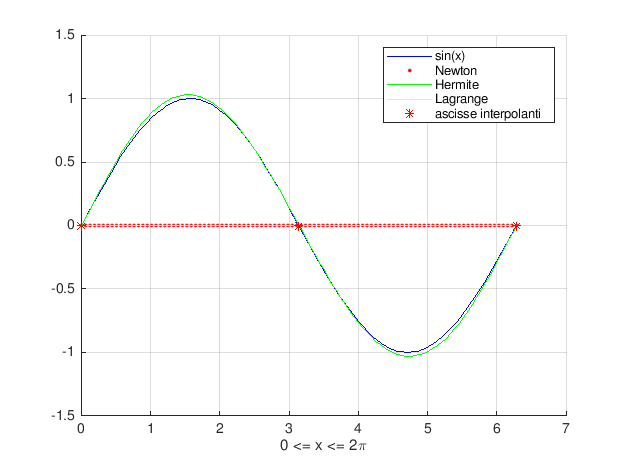
\includegraphics[width=\textwidth,height=\textheight,keepaspectratio]{Codici/Cap4/es4_cap4.png}
\end{figure}

\noindent Essendo \(f_i=0\) per tutte le ascisse \(x_i\), sia il polinomio interpolante di Lagrange, che quello di Newton in realt\'a sono la retta \(y=0\). \\ \\
\newpage
\subsection{}
\begin{center}
\large\noindent\fbox{
	\parbox{\textwidth}{
	Scrivere una function Matlab che implementi la \textit{spline} cubica interpolante (naturale o \textit{not-a-knot}, come specificato in ingresso) delle coppie di dati assegnate. La forma della function deve essere del tipo: \lstinline[language=Matlab]{y = spline3( xi, fi, x, tipo)}
	}
}\end{center}

\noindent I seguenti codici Matlab, contengono la soluzione al problema dato:

\lstinputlisting[language=Matlab]{Codici/Cap4/spline3.m}

\pagebreak

\lstinputlisting[language=Matlab]{Codici/Cap4/diffDivise.m}

\vspace*{0.5cm}

\lstinputlisting[language=Matlab]{Codici/Cap4/solveSplineNat.m}

\pagebreak

\lstinputlisting[language=Matlab]{Codici/Cap4/solveSplineNaK.m}

\pagebreak

\lstinputlisting[language=Matlab]{Codici/Cap4/createSpline.m}

\vspace*{0.5cm}

\lstinputlisting[language=Matlab]{Codici/Cap4/evaluateSpline.m}
\newpage
\subsection{}
\begin{center}
\large\noindent\fbox{
	\parbox{\textwidth}{
	Scrivere una function Matlab che implementi il calcolo delle ascisse di Chebyshev per il polinomio interpolante di grado \textit{n}, su un generico intervallo \([a, b]\). \\ \\La function deve essere del tipo: \lstinline[language=Matlab]{ xi = ceby( n, a, b )}
	}
}\end{center}

\noindent Il seguente codice Matlab implementa la function richiesta.

\lstinputlisting[language=Matlab]{Codici/Cap4/ceby.m}
\subsection{}
\begin{center}
\large\noindent\fbox{
	\parbox{\textwidth}{
	Utilizzare le function degli Esercizi 4.1 e 4.6 per graficare l'approssimazione della funzione di Runge sull'intervallo \([-6, 6]\), per \(n = 2, 4, 6, \ldots, 40\). Stimare numericamente l'errore commesso in funzione del grado \textit{n} del polinomio interpolante.
	}
}\end{center}

\noindent Il seguente codice Matlab implementa la soluzione al problema dato: 
\lstinputlisting[language=Matlab]{Codici/Cap4/Esercizio7_Cap4.m}
\vspace*{1cm}
\noindent Il grafico seguente mostra i polinomi interpolanti di grado \textit{n}, calcolati utilizzando come punti di interpolazione quelli corrispondenti alle \textit{n} ascisse di Chebyshev. Si ricorda la funzione di Runge scritta come:  \(f(x) = \frac{1}{1+25x^2}\). \\

\hspace{3.5cm}

\begin{figure}[H]
	\centering
    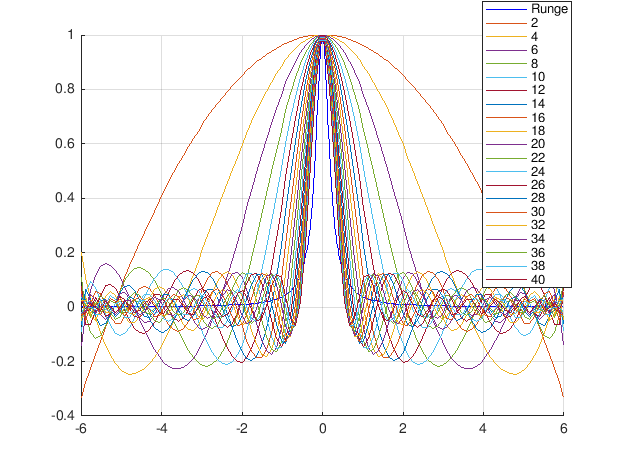
\includegraphics[width=\textwidth,height=\textheight,keepaspectratio]{Codici/Cap4/es7_cap4.png}
\end{figure}

\pagebreak
\noindent Abbiamo quindi calcolato l'errore al variare di $n$ (con $f$ = funzione di Runge e $p_n(x)$ = il suo polinomio interpolante di grado $n$) come segue:

$$
||err|| \approx ||f(x) - p_n(x)||_{\inf}
$$

\noindent Nella seguente tabella si riportano gli errori calcolati: 

\begin{center}
	\begin{tabular}{|c|c|}
		\hline
		$n$ & $\|err\|$ \\
		\hline
		$2$  & $0.9244$ \\
		$4$  & $0.8717$ \\
		$6$  & $0.8217$ \\
		$8$  & $0.7757$ \\
		$10$ & $0.7262$ \\
		$12$ & $0.6866$ \\
		$14$ & $0.6464$ \\
		$16$ & $0.6025$ \\
		$18$ & $0.5568$ \\
		$20$ & $0.5291$ \\
		$22$ & $0.5000$ \\
		$24$ & $0.4696$ \\
		$26$ & $0.4384$ \\
		$28$ & $0.4067$ \\
		$30$ & $0.3747$ \\
		$32$ & $0.3427$ \\
		$34$ & $0.3110$ \\
		$36$ & $0.2855$ \\
		$38$ & $0.2713$ \\
		$40$ & $0.2570$ \\
		\hline
	\end{tabular}
\end{center} 


\noindent Grazie alla scelta delle ascisse di Chebyshev come punti di interpolazione, l'errore diminuisce all'aumentare di \(n\).
\newpage
\subsection{}
\begin{center}
\large\noindent\fbox{
	\parbox{\textwidth}{
	Relativamente al precedente esercizio, stimare numericamente la crescita della costante di Lebesgue.
	}
}\end{center}

\noindent I seguenti codici Matlab contengono il calcolo della costante di Lebesgue in funzione di $n$. La costante di Lebesgue è definita come segue:

\[
\Lambda_n = ||\lambda_n|| \quad con \ \lambda_n(x) = \sum_{i=0}^{n} |L_{(i,n)}(x)|
\]

\lstinputlisting[language=Matlab]{Codici/Cap4/Esercizio8_Cap4.m}

\lstinputlisting[language=Matlab]{Codici/Cap4/computeLeb.m}
\pagebreak

\noindent Nella seguente tabella viene mostrata come varia la costante di Lebesgue in funzione di $n$. Come si può notare, grazie alle ascisse di Chebyshev, si ha una crescita logaritmica della costante al variare del grado n del polinomio: 

\begin{center}
	\begin{tabular}{|c|c|}
		\hline
		$n$ & $lebesgue$ \\
		\hline
		$2$  & $1.2500$ \\ 
		$4$  & $1.5702$ \\ 
		$6$  & $1.7825$ \\ 
		$8$  & $1.9416$ \\ 
		$10$ & $2.0687$ \\ 
		$12$ & $2.1747$ \\ 
		$14$ & $2.2655$ \\ 
		$16$ & $2.3450$ \\ 
		$18$ & $2.4156$ \\ 
		$20$ & $2.4792$ \\ 
		$22$ & $2.5370$ \\ 
		$24$ & $2.5900$ \\ 
		$26$ & $2.6386$ \\ 
		$28$ & $2.6843$ \\ 
		$30$ & $2.7266$ \\ 
		$32$ & $2.7662$ \\ 
		$34$ & $2.8036$ \\ 
		$36$ & $2.8391$ \\ 
		$38$ & $2.8718$ \\ 
		$40$ & $2.9022$ \\ 
		\hline
	\end{tabular}
\end{center} 


\newpage
\subsection{}
\begin{center}
\large\noindent\fbox{
	\parbox{\textwidth}{
	Utilizzare la function dell'Esercizio 4.1 per approssimare la funzione di Runge sull'intervallo \([-6,6]\), su una partizione uniforme di \(n+1\) ascisse per \(n = 2,4,6, \ldots,40\). Stimare le corrispondenti costanti di Lebesgue.
	}
}\end{center}

\noindent Il seguente codice Matlab contiene la soluzione al problema dato:

\lstinputlisting[language=Matlab]{Codici/Cap4/Esercizio9_Cap4.m}

\pagebreak
\noindent Di seguito i grafici mostrano i polinomi interpolanti di Lagrange al variare del grado  $N$ con \(N = 2,4,6, \ldots,40\).

\begin{figure}[H]
	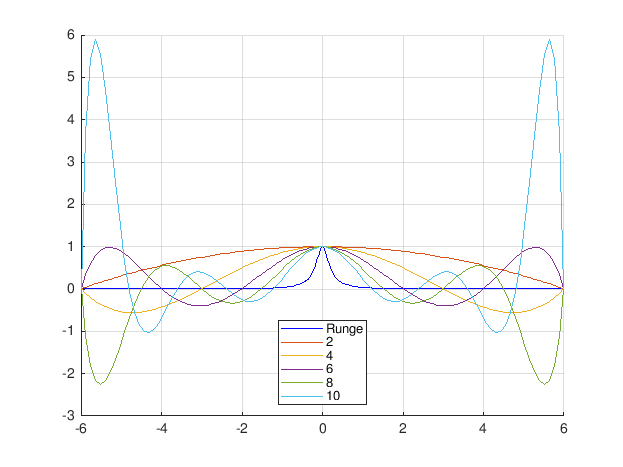
\includegraphics[height=0.6\textwidth,width=\textwidth]{Codici/Cap4/es9(n10)}
\end{figure}

\begin{figure}[H]
	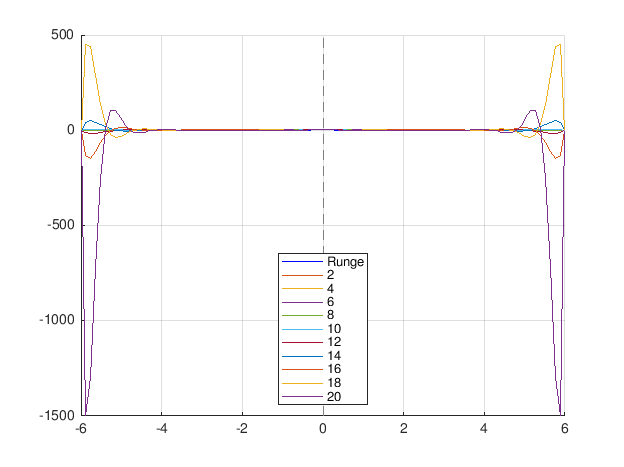
\includegraphics[width=\textwidth]{Codici/Cap4/es9(n20)}
\end{figure}

\begin{figure}[H]
	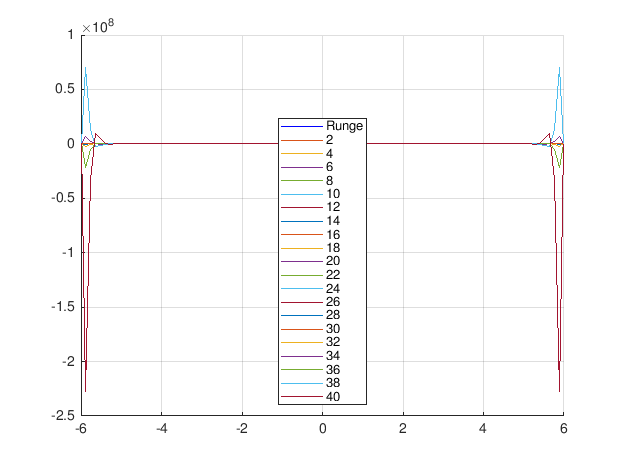
\includegraphics[height=0.6\textwidth,width=\textwidth]{Codici/Cap4/es9(n40)}
\end{figure}

Nella tabella è riportato come varia la \textit{costante di Lebesgue}, al variare del grado \textit{n} del polinomio interpolante. Come si può vedere, all'aumentare di \textit{n} l'errore aumenta a causa della scelta delle ascisse equispaziate.

\begin{center}
	\begin{tabular}{|c|c|}
		\hline
		$n$ & $lebesgue$ \\
		\hline
		$2$  & $0.9342$ \\ 
		$4$  & $0.8566$ \\ 
		$6$  & $0.9846$ \\ 
		$8$  & $2.2590$ \\ 
		$10$ & $5.8960$ \\ 
		$12$ & $16.3788$ \\ 
		$14$ & $49.2750$ \\ 
		$16$ & $147.6550$ \\ 
		$18$ & $450.3933$ \\ 
		$20$ & $1.5025e+03$ \\ 
		$22$ & $5.0066e+03$ \\ 
		$24$ & $1.6654e+04$ \\ 
		$26$ & $5.5282e+04$ \\ 
		$28$ & $1.8307e+05$ \\ 
		$30$ & $6.0468e+05$ \\ 
		$32$ & $1.9918e+06$ \\ 
		$34$ & $6.5422e+06$ \\ 
		$36$ & $2.1426e+07$ \\ 
		$38$ & $6.9960e+07$ \\ 
		$40$ & $2.2774e+08$ \\ 
		\hline
	\end{tabular}
\end{center}
\newpage
\subsection{}
\begin{center}
\large\noindent\fbox{
	\parbox{\textwidth}{
	Stimare, nel senso dei minimi quadrati, posizione, velocit\'a iniziale ed accelerazione relative ad un moto rettilineo uniformemente accelerato per cui sono note le seguenti misurazioni dele coppie \((tempo, spazio)\):\\
	\((1, 2.9) \quad (1, 3.1)\quad (2, 6.9) \quad (2, 7.1) \quad (3, 12.9) \quad (3, 13.1) \quad (4, 20.9) \quad (4, 21.1) \quad (5, 30.9) \quad (5, 31.1)\)
	}
}\end{center}

\noindent La legge che descrive il fenomeno del moto rettilineo uniformemente accelerato si pu\'o scrivere in forma polinomiale come segue:

\[
y =  s(t) = x_0 + v_0t + a_0t^2 \quad \quad \text{con } a_0 = \frac{1}{2}a
\]

\noindent Il cui grado è n = 2. Il sistema ha soluzione se si ha almeno n+1 punti distinti.
In questo caso il problema \'e ben posto poich\'e i punti distinti sono 5>3.

\noindent Si vuole quindi stimare nel senso dei minimi quadrati: posizione, velocità iniziale, ed accelerazione, che equivale alla risoluzione del sistema lineare sovradeterminato:
\[
V\underline{a}=\underline{y}
\]

\noindent con $V$ matrice di tipo \textit{Vandermonde} (la trasposta di una matrice di tipo Vandermonde), \underline{a} vettore delle incognite e  \underline{y} il vettore dei valori misurati. \\
\noindent Tale sistema si risolve mediante fattorizzazione \textit{QR}. La matrice $V$ è scritta come segue: 

\[
V=\begin{bmatrix}
x_0^0 & x_0^1 & \cdots & x_0^m \\
x_1^0 & x_1^1 & \cdots & x_1^m \\
\vdots & \vdots & & \vdots \\
x_n^0 & x_n^1 & \cdots & x_n^m \\		
\end{bmatrix}
\]
\vspace*{0.5cm}

\lstinputlisting[language=Matlab]{Codici/Cap4/SoluzioneEs10_Cap4.m}

\noindent Le soluzioni, calcolate, al problema dato sono :
\begin{center}
	$x_0 = 1$, $v_0 = 1$, $a_0 = 1$ 
\end{center}

	\newpage
	\vspace{0.8cm}
\section{\textbf{Capitolo}}
\subsection{}
\large\noindent\fbox{
	\parbox{\textwidth}{
	Determinare analiticamente gli zeri del polinomio $P(x)=x^3 -4x^2 + 5x -2$ e la loro molteplicità.
	Dire perchè il metodo di bisezione è utilizzabile per approssimarne uno a partire dall’intervallo di confidenza \textit{[a , b] = [0 , 3]}. A quale zero di \textit{P} potrà tendere la successione generata dal metodo di bisezione a partire da tale intervallo? Costruire una tabella in cui si riportano il numero di iterazioni e di valutazioni di P richieste per valori decrescenti della tolleranza tolx.
	}}

Studio analitico del polinomio $P(x) = x^3-4x^2+5x-2$.\\
\begin{itemize}
	\item \textbf{Zeri del polinomio}\\
		Per trovare gli zeri del polinomio occorre scomporlo nel seguente modo:
			\[
			\ x^3-4x^2+5x-2 =
			\] 
			\[
			\ = (x-2)(x^2-2x+1) =
			\]
			\[
			\ = (x-2)(x-1)^2
			\]\\
		Da cui si deduce che $P(x)=0$ per $(x-2)=0 \Rightarrow x=2$ e $(x-1)=0 \Rightarrow x=1$. \\
	\item \textbf{Molteplicità}\\
		I valori di \textit{x} precedentemente calcolati vengono definiti come \textit{radici} del polinomio. Si dice che \textit{a} è una radice di \textit{P(x)} con \textit{molteplicità n} se e solo se \textit{P(x)} è divisibile per $(x-a)^n$, ma non è divisibile per $(x-a)^{n-1}$.\\
		Inoltre si dice che \textit{x} ha \textit{molteplicità esatta} $n \geq 1$, se:
			\[
			f(x) = f'(x) = ... = f^{(n-1)}(x) = 0,  f^{(n)}(x) \neq 0.
			\]
				$\bullet x = 2 $ \\[0.5cm]
					\[
					P(2) = 8-16+10-2 = 0 
					\]
					\[
					P'(2) = 3x^2-8x+5 = 12-16+5 = 1 \neq 0 \Rightarrow \textit{ molteplicità } n=1
					\]\\
				$\bullet x = 2 $ \\[0.5cm]
					\[
					P(1) = 1-4+5-2 = 0 
					\]
					\[
					P'(1) = 3x^2-8x+5 = 3-8+5 = 0 
					\]
					\[
					P''(1) = 6x-8 = 6-8 \neq 0 \Rightarrow \textit{ molteplicità } n=2
					\]
		In questo caso la radice $x=2$ viene definita \textit{semplice} in quanto ha molteplicità $m=1$,
mentre la radice $x=1$ si definisce \textit{multipla} data la molteplicità $m=2$.\\ 
\end{itemize}
Il requisito per poter applicare il \textit{metodo di bisezione} in un intervallo $[a,b]$ è che sia $f(a)f(b)<0$ in modo da garantire l'esistenza di almeno uno zero. Per il polinomio $P(x)$ è possibile applicare il \textit{metodo di bisezione} nell'intervallo $[0,3]$ poichè il requisito è soddisfatto.
In questo caso si ha: $P(0)*P(3) = (-2)*(4) = -8$.\\\\
Il seguente codice MatLab, riguarda il \textbf{Metodo di bisezione}:\\
	\lstinputlisting[language=Matlab]{Codici/Cap2/Bisezione_Es1.m}
Nel seguente codice Matlab viene applicato il \textit{metodo di bisezione} al polinomio $P(x)$ sull'intervallo $[0,3]$, con una tolleranza iniziale pari a $10^-1$, la quale viene decremntata di un fattore $10$ ad ogni iterazione:\\
	\lstinputlisting[language=Matlab]{Codici/Cap2/Es1_cap2.m}
Da i seguenti valori riportati dall'esecuzione del codice è possibile notare che la successione generata dal metodo di \textit{bisezione} converge alla radice $x = 2$:\\
\begin{center}
	\begin{tabular}{|c|c|c|}
		\hline
			$tol_x$ & \textit{Bisezione} & \textit{Num. Iterazioni} \\
		\hline
   			$10^{-1}$ & $\tilde{x} = 1.500000000000000$ & $ib = 0$\\
    		$10^{-2}$ & $\tilde{x} = 1.992187500000000$ & $ib = 6$\\
    		$10^{-3}$ & $\tilde{x} = 2.000976562500000$ & $ib = 9$\\
    		$10^{-4}$ & $\tilde{x} = 2.000061035156250$ & $ib = 13$\\
   			$10^{-5}$ & $\tilde{x} = 1.999992370605469$ & $ib = 16$\\
   			$10^{-6}$ & $\tilde{x} = 2.000000953674316$ & $ib = 19$\\
    		$10^{-7}$ & $\tilde{x} = 2.000000059604645$ & $ib = 23$\\
    		$10^{-8}$ & $\tilde{x} = 1.999999992549419$ & $ib = 26$\\
    		$10^{-9}$ & $\tilde{x} = 2.000000000931323$ & $ib= 29$\\
    		$10^{-10}$ & $\tilde{x} = 2.000000000058208$ & $ib = 33$\\
    		$10^{-11}$ & $\tilde{x} = 1.999999999992724$ & $ib = 36$\\
    		$10^{-12}$ & $\tilde{x} = 2.000000000000910$ & $ib = 39$\\
    		$10^{-13}$ & $\tilde{x} = 2.000000000000057$ & $ib = 43$\\
    		$10^{-14}$ & $\tilde{x} = 1.999999999999993$ & $ib = 46$\\
    		$10^{-15}$ & $\tilde{x} = 2.000000000000001$ & $ib = 49$\\
		\hline
	\end{tabular}
\end{center}
\newpage
\subsection{}
\large\noindent\fbox{
	\parbox{\textwidth}{
	Scrivere una function Matlab che implementi la formula composita di Simpson su $2n + 1$ ascisse equidistanti nell’intervallo \textit{[a, b]}, relativamente alla funzione implementata da \textbf{fun(x)}. La function deve essere del tipo: \textbf{If = simpcomp( n, a, b, fun )}.
}}\\[0.5cm]

Il codice riportato in seguito implementa la formula \textit{composita di Simpson} su $2n+1$ ascisse
equidistanti definite sull'intervallo \textit{[a,b]}, relativa alla generica funzione $fun(x)$ e ne 
restiusce l'approssimazione del relativo integrale.
\lstinputlisting[language=Matlab]{Codici/Cap5/simpcomp.m}
\newpage
\subsection{}
\large\noindent\fbox{
	\parbox{\textwidth}{
	Scrivere una function Matlab che implementi la formula composita dei trapezi adattativa nell’intervallo \textit{[a, b]}, relativamente alla funzione implementata da \textbf{fun(x)}, e con tolleranza \textbf{tol}. La function deve essere del tipo:
	\textbf{If = trapad( a, b, fun, tol )}.
}}\\[0.5cm]

Il codice riportato in seguito implementa la formula \textit{adattiva dei trapezi} sull'intervallo  \textit{[a,b]},
relativa alla generica funzione fun(x), con una tolleranza tol e ne 
restiusce l'approssimazione del relativo integrale.\\
\lstinputlisting[language=Matlab]{Codici/Cap5/trapad.m}
\newpage
\subsection{}
\large\noindent\fbox{
	\parbox{\textwidth}{
	Definire una procedura iterativa basata sul metodo di Newton per approssimare $\sqrt{\alpha}$, per un assegnato $\alpha > 0$. Costruire una tabella dove si riportano le successive approssimazioni ottenute e i corrispondenti errori assoluti (usare l’approssimazione Matlab di $\sqrt{\alpha}$ per il calcolo dell’errore) nel caso in cui $\sqrt{\alpha} = 5$ partendo da $x_{0} = 5$.
	}}\\

Dato che  $\sqrt{\alpha}$ è la radice ricercata, occorre quindi trovare una
funzione $f(x)$ che abbia uno \textit{zero} in appunto $\sqrt{\alpha}$.
La funzione ricercata in questo caso è $f(x) = x^2 - \alpha$, la quale ha due radici
semplici in $\pm\sqrt{\alpha}$ e ha derivata $f'(x) = 2x$.\\\\
L'iterazione del metodo di Newton utilizzando questa funzione diventa :
	\[
	x_{i+1} = x_i-\frac{f(x_i)}{f'(x_i)} = x_i - \frac{x_i^2-\alpha}{2x_i} =
	\]
	\[
	= \frac{2x_i^2-x_i^2+\alpha}{2x_i} = \frac{x_i^2+\alpha}{2x_i} =
	\]
	\[
	= \frac{1}{2} \Bigl( x_i+\frac{\alpha}{x_i} \Bigl),\quad i=0,1,2,...
	\]\\\\
Il seguente codice MatLab, riguarda l'implementazione del \textbf{metodo di Newton per il calcolo} $\sqrt{\alpha}$:\\ 
	\lstinputlisting[language=Matlab]{Codici/Cap2/newtonSolveEs4.m}
Il seguente codice MatLab, riguarda la chiamata della funzione definita precedentemente, con $\alpha=x_0=5$, con numero di passi massimi $itmax=10$ e indice di tolleranza $tol_x=eps$ :\\
	\lstinputlisting[language=Matlab]{Codici/Cap2/Es4_cap2.m}
restituisce i seguenti valori:\\
\begin{center}
	\begin{tabular}{|c|c|c|}
		\hline
			$i$ & $x_i$ & $E_{ass}=\epsilon_i=|x_i-\sqrt{\alpha}| \quad \alpha=5$ \\
		\hline
    		$i=0$ & $x_0 = 5$ & $|\epsilon_0| = 2.763932022500210$\\
    		$i=1$ & $x_1 = 3$ & $|\epsilon_1| = 0.763932022500210$\\
    		$i=2$ & $x_2 = 2.333333333333334$ & $|\epsilon_2| = 0.097265355833544$\\
    		$i=3$ & $x_3 = 2.238095238095238$ & $|\epsilon_3| = 0.002027260595448$\\
    		$i=4$ & $x_4 = 2.236068895643363$ & $|\epsilon_4| = 9.181435736138610e-07$\\
    		$i=5$ & $x_5 = 2.236067977499978$ & $|\epsilon_5| = 1.882938249764266e-13$\\
    		$i=6$ & $x_6 = 2.236067977499790$ & $|\epsilon_6| = 0$\\
    		$i=7$ & $x_7 = 2.236067977499790$ & $|\epsilon_7| = 0$\\
		\hline
	\end{tabular}
\end{center}
\newpage
\subsection{}
\large\noindent\fbox{
	\parbox{\textwidth}{
	Definire una procedura iterativa basata sul metodo delle secanti sempre per approssimare $\sqrt{\alpha}$, per un assegnato $\alpha > 0$. Completare la tabella precedente aggiungendovi i risultati ottenuti con tale procedura partendo da $x_{0} = 5$ e $x_{1} = 3$. Commentare i risultati riportati in tabella.
	}}\\

Come visto nel precedente esercizio occorre utilizzare la funzione $f(x) = x^2 - \alpha$\\
L'iterazione del metodo delle Secanti utilizzando questa funzione diventa:
	\[
	x_{i+1} = \frac{f(x_i)x_{i-1}-f(x_{i-1})x_i}{f(x_i)-f(x_{i-1})} =
	\]
	\[
	= \frac{(x_i^2-\alpha)x_{i-1}-(x_{i-1}^2-\alpha)x_i}{x_i^2-\alpha-x_{i-1}^2+\alpha}  =
	\]
	\[
	= \frac{x_i^2x_{i-1}-\alpha x_{i-1}-x_{i-1}^2x_i+\alpha x_i}{x_i^2-x_{i-1}^2} =
	\]
	\[
	= \frac{x_ix_{i-1}(x_i-x_{i-1})+\alpha (x_i-x_{i-1})}{(x_i-x_{i-1})(x_i+x_{i-1})} =
	\]
	\[
	= \frac{(x_i-x_{i-1})(x_ix_{i-1}+\alpha)}{(x_i-x_{i-1})(x_i+x_{i-1})} =
	\]
	\[
	= \frac{x_ix_{i-1}+\alpha}{x_i+x_{i-1}},\quad i=0,1,2,...
	\]\\
L'implementazione del metodo delle secanti in Matlab è la seguente:\\ 
	\lstinputlisting[language=Matlab]{Codici/Cap2/secantiSolveEs5.m}
Il seguente codice MatLab, riguarda la chiamata della funzione definita precedentemente, con $\alpha=x_0=5$, con $x_1=3$, con numero di passi massimi $imax=100$ e indice di tolleranza $tol_x=eps$ :\\
	\lstinputlisting[language=Matlab]{Codici/Cap2/Es5_Cap2.m}
restituisce i seguenti valori:\\
\begin{center}
	\begin{tabular}{|c|c|c|}
		\hline
			$i$ & $x_i$ & $E_{ass}=\epsilon_i=|x_i-\sqrt{\alpha}| \quad \alpha=5$ \\
		\hline
    		$i=0$ & $x_0 = 5$ & $|\epsilon_0| = 2.763932022500210$\\
    		$i=1$ & $x_1 = 3$ & $|\epsilon_1| = 0.763932022500210$\\
    		$i=2$ & $x_2 = 2.500000000000000$ & $|\epsilon_2| = 0.263932022500210$\\
    		$i=3$ & $x_3 = 2.272727272727273$ & $|\epsilon_3| = 0.36659295227483$\\
    		$i=4$ & $x_4 = 2.238095238095238$ & $|\epsilon_4| = 0.00202760595448$\\
    		$i=5$ & $x_5 = 2.236084452975048$ & $|\epsilon_5| = 1.647547525829296e-05$\\
    		$i=6$ & $x_6 = 2.236067984964863$ & $|\epsilon_6| = 7.465073448287285e-09$\\
    		$i=7$ & $x_7 = 2.236067977499817$ & $|\epsilon_7| = 2.753353101070388e-14$\\
    		$i=8$ & $x_8 = 2.236067977499790$ & $|\epsilon_8| = 4.440892098500626e-16$\\
    		$i=9$ & $x_9 = 2.236067977499790$ & $|\epsilon_9| = 0$\\
    		$i=10$ & $x_{10} = 2.236067977499790$ & $|\epsilon_{10}| = 0$\\
		\hline
	\end{tabular}
\end{center}
\newpage
	\newpage
	\vspace{0.8cm}
\section{\textbf{Capitolo}}
\subsection{}
\begin{center}
\large\noindent\fbox{
	\parbox{\textwidth}{
	  Scrivere una function Matlab che generi la matrice \textit{sparsa} $n \times n$, con $n > 10$

$$
A_n = \begin{pmatrix} a_{11} & \ldots & a_{1n} \\ \vdots & & \vdots \\ a_{n1} & \ldots & a_{nn}\end{pmatrix} \text {, con } a_{ij} =  \begin{cases} 4 \text{ se } i = j \\ -1 \text{ se } i = j \pm 1 \\ -1 \text{ se } i = j \pm 10\end{cases}
$$

Utilizzare,a questo fine, la function Matlab spdiags.
}
}\end{center}

\noindent Il seguente codice Matlab risolve il problema dato utilizzando la funzione \lstinline[language=Matlab]{spdiags}:

\lstinputlisting[language=Matlab]{Codici/Cap6/createSparseMatrix.m}
\newpage
\subsection{}
\begin{center}
\large\noindent\fbox{
	\parbox{\textwidth}{
    Utilizzare il metodo delle potenze per calcolarne l'autovalore dominante della matrice $A_n$ del precedente esercizio, con una approssimazione $tol=10^{-5}$, partendo da un vettore con elementi costanti. Riempire, quindi, la seguente tabella: \\ \begin{center}
  \begin{tabular}{ | l | c | r |}
    \hline
    $n$ & \textit{numero iterazioni effettuate} & \textit{stima autovalore} \\ \hline
    100 &  &  \\ 
    200 &  &  \\ 
    \vdots &  &  \\  
	1000 &  &  \\
    \hline
  \end{tabular}
\end{center}
}
}\end{center}
\noindent Di seguito sono riportati i codici implementati. La funzione \textit{potenze} calcola sia l'autovalore dominante della matrice \textit{A} , sia il numero di iterazioni, \textit{numIt }, impiegate.
\vspace{0.5cm}

\lstinputlisting[language=Matlab]{Codici/Cap6/SoluzioneEs2_Cap6.m}
\lstinputlisting[language=Matlab]{Codici/Cap6/potenze.m}

\noindent Nella seguente tabella \'e possibile visualizzare i risultati ottenuti: 

\begin{center}
	\begin{tabular}{ | l | c | c |}
		\hline
		$n$ & \textit{numero iterazioni effettuate} & \textit{stima autovalore} \\ \hline
		$100$ & $167$ & $7.8224$ \\
		$200$ & $420$ & $7.8803$ \\
		$300$ & $638$ & $7.8916$ \\
		$400$ & $721$ & $7.8949$ \\
		$500$ & $743$ & $7.8964$ \\
		$600$ & $824$ & $7.8974$ \\
		$700$ & $893$ & $7.8976$ \\
		$800$ & $868$ & $7.8967$ \\
		$900$ & $795$ & $7.8957$ \\
		$1000$ & $775$ & $7.8954$ \\
		\hline
	\end{tabular}
\end{center}
\newpage
\subsection{}
\begin{center}
\large\noindent\fbox{
	\parbox{\textwidth}{
	  Utilizzare il metodo di Jacobi per risolvere il sistema lineare
	  $$
	  A_n \textbf{x} = \begin{pmatrix} 1 \\ \vdots \\ 1 \end{pmatrix}
	  $$

	  dove $A_n$ è la matrice definita nell'Esercizio 6.1, con tolleranza $tol=10^{-5}$, e partendo dal vettore nullo. Graficare il numero di iterazioni necessarie, rispetto alla dimensione $n$ del problema, con $n$ che varia da 100 a 1000 (con passo 20).
}
}\end{center}

\noindent Di seguito si riportano i codici Matlab utilizzati. La funzione di \textit{Jacobi} oltre ad effettuare il calcolo del vettore delle incognite della matrice $A$, restituisce anche il numero di iterazioni \textit{numIt} impiegate e la norma infinito del residuo, al passo i-simo.

\lstinputlisting[language=Matlab]{Codici/Cap6/SoluzioneEs3_Cap6.m}
\vspace*{0.5cm}
\lstinputlisting[language=Matlab]{Codici/Cap6/jacobi.m}
\vspace*{1cm}
\noindent Graficamente si pu\'o osservare il seguente risultato, al variare di \textit{n}: 

\begin{figure}[H]
	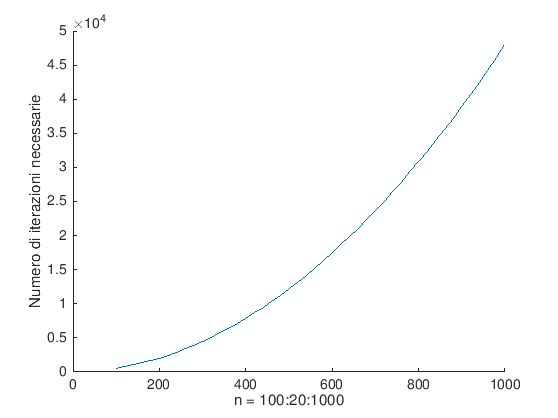
\includegraphics[width=\textwidth]{Codici/Cap6/es3_cap6}
\end{figure}
\newpage
\subsection{}
\begin{center}
\large\noindent\fbox{
	\parbox{\textwidth}{
	 Ripetere una procedura analoga a quella del precedente esercizio utilizzando il metodo di Gauss-Seidel.
}
}\end{center}

\noindent Il codice Matlab utilizzato per realizzare il grafico \'e il seguente:

\lstinputlisting[language=Matlab]{Codici/Cap6/Soluzione4_Cap6.m}

\vspace*{0.5cm}

\lstinputlisting[language=Matlab]{Codici/Cap6/gaussSeidel.m}

\vspace*{0.5cm}

\lstinputlisting[language=Matlab]{Codici/Cap6/trisolveInfGaussSeidel.m}

\noindent Grafico risultante: 

\begin{figure}[H]
	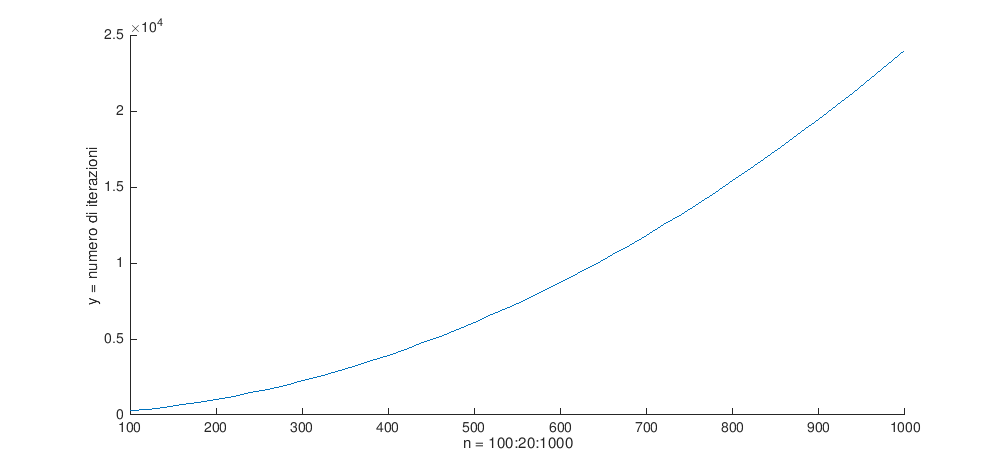
\includegraphics[width=\textwidth]{Codici/Cap6/es4cap6}
\end{figure}

\newpage
\subsection{}
\begin{center}
\large\noindent\fbox{
	\parbox{\textwidth}{
Con riferimento al sistema lineare dell' Esercizio 6.3, con $n=1000$, graficare la norma dei residui, rispetto all'indice di iterazione, generati dai metodi di Jacobi e Gauss-Seidel. Utilizzare il formato \textit{semilogy} per realizzare il grafico, corredandolo di opportune $label$.
} }
\end{center}

\noindent Il seguente codice Matlab \'e stato utilizzato per la risoluzione del problema:

\lstinputlisting[language=Matlab]{Codici/Cap6/SoluzioneEs5_Cap6.m}

\vspace*{1cm}

\noindent Il grafico seguente mostra la norma dei residui, rispetto all'indice di iterazione generati dai metodi di Jacobi (in azzurro) e Gauss-Seidel (in rosso):


\begin{figure}[H]
	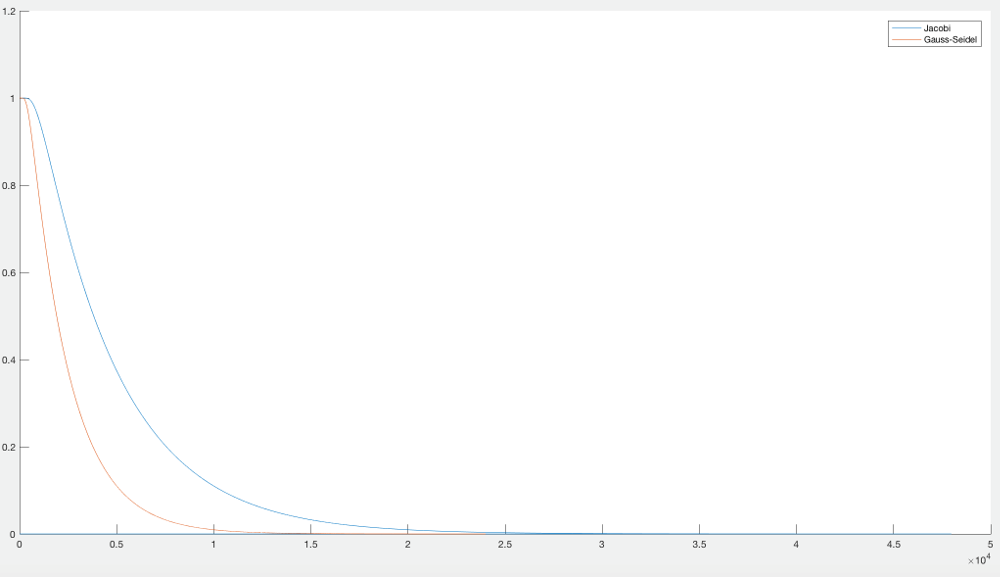
\includegraphics[width=\textwidth]{Codici/Cap6/Es5_Cap61}
\end{figure}
\newpage
    \newpage

	
\end{document}